\documentclass{article}

% NeurIPS 2026 Main Track, double-blind submission
% (environ dependency removed; \NewEnviron in style file replaced with \newenvironment fallback for legacy TexLive 2020 compat)
\usepackage{neurips_2026}

\usepackage[utf8]{inputenc}
\usepackage[T1]{fontenc}
\usepackage{hyperref}
\usepackage{url}
\usepackage{booktabs}
\usepackage{amsmath}
\usepackage{amssymb}
\usepackage{amsfonts}
\usepackage{graphicx}
% nicefrac removed: not available in TexLive 2020 minimal install
% \usepackage{nicefrac}
\usepackage{microtype}
\usepackage{xcolor}
\usepackage{tikz}
\usetikzlibrary{arrows.meta, positioning, shapes.geometric, calc}

\newcommand{\method}{Envisage}
\newcommand{\best}[1]{\textbf{#1}}
\newcommand{\second}[1]{\underline{#1}}

\title{Envisage: Diffusion-Based Rhinoplasty Goal Visualization with Mask-Decomposed Evaluation}

% Double-blind submission: author block is anonymous.
% Do NOT fill in author names, affiliations, or emails before submission.
\author{Anonymous}

% Relax line-breaking around long \texttt{} paths to avoid wide inter-word
% gaps in justified paragraphs.
\emergencystretch=3em
\hyphenpenalty=200
\tolerance=2000

\begin{document}

\maketitle

%% ========================================================================
%% ABSTRACT
%% ========================================================================
\begin{abstract}
Localized generative editing needs localized evaluation: full-image identity
metrics are structurally confounded under hard-composited edits. We present
\textbf{\method{}}, a FLUX.1-Fill inpainting reference pipeline for
rhinoplasty goal visualization from a single frontal photograph. The
pipeline combines $24$ landmark-indexed clinical presets, MediaPipe masks,
and hard-mask compositing. The composite preserves outside-mask pixels by
construction, so full-face identity scores are dominated by copied pixels
rather than by the diffusion backbone. We therefore introduce
\textbf{SurgicalScore}, a mask-decomposed $0$--$1$ protocol scoring edit
direction, edit magnitude, masked LPIPS, realism, and outside-mask SSIM;
its raw composite assigns $0.919$ $[0.918, 0.920]$ to a perfect-predictor
control, anchoring the ceiling.

On $N{=}211$, the paired ArcFace gain (output-to-GT minus
input-to-GT) is negative for all methods (\method{} $-0.048$ smallest,
vs.\ ICEdit $-0.139$, Kontext $-0.242$, InstructPix2Pix $-0.294$;
$p<10^{-4}$), with external validation on a $457$-pair ASPS/PCA corpus
showing the same negative gap. This decrease is due to the in-mask edit
failing to shift identity toward post-op: copied outside-mask pixels
are identical between input and output, so the paired difference is
dominated by the in-mask shift. With SurgicalScore, \method{} achieves
the highest score ($0.599$ $[0.579, 0.619]$); the divergence from the
ArcFace ranking suggests global identity is the wrong proxy for localized
surgical accuracy. Furthermore, a $5$-seed oracle reduces the residual ArcFace gap by
$73\%$ ($-0.054$ to $-0.015$), with positive output-to-GT gain on $33.9\%$
of cases; SurgicalScore is also raised from $0.609$ to $0.743$
$[0.725, 0.762]$ ($N{=}207$), indicating candidate-space headroom for a
learned ranker. As such, the path forward for surgical-prediction runs through metrics
that measure the edit, not the face around it. We release
\method{}, SurgicalScore, preset definitions, and matched split manifests.
\end{abstract}

%% ========================================================================
%% 1. INTRODUCTION
%% ========================================================================
\section{Introduction}
\label{sec:intro}

Rhinoplasty accounts for approximately 180,000 procedures annually in the United
States~\citep{asps2024stats}. At this volume, expectation management is the dominant
determinant of patient satisfaction; revision rates of 5--15\%~\citep{neaman2013rhinoplasty,newman2024revision}
reflect, in part, discrepancies between expected and actual outcomes.
Current visualization tools span surgeon-drawn sketches and 2D overlays at one end
to proprietary 3D simulation systems such as Crisalix and Vectra 3D at the other.
The 3D systems require capital investment in stereophotogrammetry hardware and
dedicated capture space, plus per-clinic licensing and trained operators; these
costs restrict access to high-volume metropolitan practices and exclude solo,
rural, and community settings. Sketches and 2D overlays, on the other hand, are surgeon-dependent,
single-view, and not photorealistic. The issue is clear: we need a tool
that is believable, affordable, and faithful to the surgical scope. That
means photorealistic outputs, no specialized capture hardware, and
architectural preservation of non-surgical regions. No existing system delivers all
three.

The gap has two structural roots. First, the methods themselves fall short:
geometric methods~\citep{bookstein1989tps} cannot
synthesize new skin texture, 3D approaches require CT scans or
meshes~\citep{ma2021orthognathic} unavailable in standard clinics, and full-face
diffusion models drift identity across non-surgical regions. Second, the
metric is broken too: full-face evaluation conflates two distinct objectives
(outside-mask identity preservation and inside-mask surgical accuracy) and
reports a single number that mixes them.

LandmarkDiff~\citep{landmarkdiff_anon} established the failure mode. That
system conditioned SD~1.5 on landmark wireframes and regenerated the entire
face before compositing the surgical region back. Decomposed evaluation
showed over $95\%$ of its identity score came from copied pixels: $0.509$
composited, $0.023$ without. The result exposed five architectural
limitations: low-resolution backbone, sparse conditioning, full-face
regeneration, synthetic training data, post-hoc compositing. \method{}
corrects all five.

We invert the formulation. Rather than regenerate the full face and
composite the surgical region back, the pipeline masks the surgical region
from the outset, modifies a monocular depth map at landmark-indexed
Gaussians to encode the target tissue change, runs a pretrained
depth-conditioned diffusion model on the mask only, and composites the
output verbatim with the input outside the mask. Outside-mask identity
preservation is an architectural guarantee, not a backbone assumption: the
only quantity left to measure is inside-mask edit fidelity against paired
postoperative ground truth.

That formulation produces the smallest GT-vs-BL ArcFace gap of any method
evaluated on an $N{=}211$ ASPS+PCA cohort (\method{} $-0.048$ vs.\
ICEdit $-0.139$, Kontext $-0.242$, IP2P $-0.294$; $p<10^{-4}$ paired) and
the highest mask-decomposed SurgicalScore ($0.599$ $[0.579, 0.619]$ vs.\
$0.502$ / $0.337$ / $0.229$). The result replicates on a $457$-pair external
corpus. No method, including ours, achieves positive paired ArcFace gain
over the unedited input proxy: this is a finding about the metric, not a
failure to report. ArcFace was trained for full-face verification across
changes orders of magnitude larger than rhinoplasty; it cannot grade an
edit at $5\%$-of-pixels scale.

\paragraph{Our contributions.}
\begin{enumerate}
\item \textbf{Methodological diagnosis.} Full-image identity metrics are
structurally confounded under hard-composited edits. Outside-mask SSIM exceeds
$0.999$ for FLUX backbones wrapped in our composite
(Appendix~\ref{app:composite_full}); the property is rule-driven, not
backbone-driven, and generalizes beyond rhinoplasty
(Appendix~\ref{app:cross_proc}).
\item \textbf{SurgicalScore.} A mask-decomposed $0$--$1$ protocol scoring
landmark edit direction, magnitude, masked LPIPS, realism, and outside-mask
preservation. Released with matched HDA paired pre/post splits
($N{=}27$ bleph, $N{=}21$ rhino, $N{=}9$ rhytid). The raw composite assigns
$0.919$ $[0.918, 0.920]$ to a perfect-predictor control, anchoring the
ceiling.
\item \textbf{Cross-method, cross-procedure characterization.} No method
exceeds the input proxy under GT ArcFace on $N{=}211$. \method{} produces
the only positive-gap fraction above $5\%$ ($16.1\%$ vs.\ $0.0$ / $4.3$ /
$1.0\%$). SurgicalScore reveals component-level failure modes that ArcFace
alone hides.
\item \textbf{\method{} reference pipeline.} Depth-conditioned FLUX-Fill
inpainting with $8$ rhinoplasty presets (Daniel's taxonomy) plus $8$
blepharoplasty (Tessier) and $8$ rhytidectomy (SMAS) preset definitions
released as infrastructure. Smallest GT-vs-BL ArcFace gap and highest
SurgicalScore of any method evaluated.
\end{enumerate}

\paragraph{Component-level evidence.} On $N{=}211$ ($B{=}10{,}000$, K$=5$
best-of paired permutation), each component is individually
paired-significant: hard-mask composite $\Delta$SS$=+0.034$ ($p{=}0.001$),
$24$-preset depth modification $\Delta$SS$=+0.034$ ($p{=}0.002$),
depth-ControlNet conditioning $\Delta$SS$=+0.023$ ($p{=}0.030$,
Appendix~\ref{app:ablation}). Equipping baselines with the same composite
closes most of the bare-baseline gap; \method{} still leads
ICEdit$+$composite by $+0.058$ ($p<10^{-3}$) and IP2P$+$composite by
$+0.045$ ($p{=}0.008$, Appendix~\ref{app:composite_ablation}). K$=5$ best-of
upper-bounds the deployed-system contribution; recovering the gain requires
a learned ranker (Appendix~\ref{app:deployable_ranker}: naive rankers do
not).

%% ========================================================================
%% 2. RELATED WORK
%% ========================================================================
\section{Related Work}
\label{sec:related}

\paragraph{Surgical prediction.}
\citet{eldaly2022rhinoplastyAIreview} survey simulation and AI methods
for rhinoplasty; the surveyed geometric warp approaches cannot synthesize
new skin texture.
\citet{jung2024rhinoplastygan} train a pix2pix GAN on lateral-profile
silhouettes ($N{=}3{,}030$ pairs) and report $52.5\%$ Visual Turing Test
discrimination. Frontal and internal views are excluded by dataset
construction, leaving the frontal regime open.
\citet{bini2025facial} apply inpainting and depth estimation to facial
reconstruction, a different task from aesthetic rhinoplasty on intact
anatomy. \citet{loorduque2024septorhinoplasty} apply diffusion to
septorhinoplasty visualization but evaluate without paired ground-truth or
identity metrics. \citet{varghaei2025aesthetic} report landmark-based
aesthetic outcome assessment on $1{,}259$ paired patients ($N{=}366$
rhinoplasty), establishing the geometric-plus-identity evaluation regime
our SurgicalScore extends.
PtosisDiffusion~\citep{ptosisdiffusion2024} uses training-free ControlNet
guidance for blepharoptosis, a precedent for zero-shot surgical
simulation; we extend it to depth-conditioned blepharoplasty, rhinoplasty,
and rhytidectomy. 3D methods~\citep{ma2021orthognathic} require volumetric or
multi-view input, unavailable in standard clinics.

\paragraph{Diffusion models and ControlNet.}
Latent diffusion models~\citep{rombach2022latent} generate photorealistic
images from text and spatial conditioning; ControlNet~\citep{zhang2023controlnet}
adds spatial control to frozen backbones via zero-convolution layers. Depth
conditioning maps tissue displacement directly to surface change, a
connection edge or pose conditioning does not provide.
ICEdit~\citep{zhang2025icedit} applies instruction-based editing via
FLUX.1-Fill-dev with a mixture-of-experts LoRA and a diptych formulation; we
evaluate it as a baseline (Section~\ref{sec:results}).

\paragraph{Identity preservation.}
ArcFace~\citep{deng2019arcface} cosine similarity is the standard identity
metric in face research. It conflates identity change in the surgical
region (expected) with identity drift in non-surgical regions (undesired);
our mask-decomposed evaluation separates these terms. Face-recognition
fairness on darker skin tones is documented in the broader
literature~\citep{buolamwini2018gender}, but no prior surgical-prediction
work reports metrics stratified by the Monk Skin Tone
Scale~\citep{monk2023monk}.

%% ========================================================================
%% 3. METHODS
%% ========================================================================
\section{Methods}
\label{sec:methods}

\subsection{Pipeline Overview}

We invert the formulation: \method{} masks the surgical region from the
outset rather than regenerating the full face and compositing the surgical
region back. A procedure-specific text prompt provides the semantic
direction of change; a modified monocular depth map encodes the intended
surface displacement. After denoising, a hard-mask composite copies all
non-surgical pixels verbatim from the input.

Outside-mask identity preservation is an architectural guarantee, not a
backbone assumption. The remaining modeling problem is inside the mask:
edit fidelity against paired postoperative ground truth.

The three pipeline stages are: (1)~\emph{TPS pre-warp} for procedure-specific
geometric deformation; (2)~\emph{depth modification} to encode profile changes
on the monocular depth map; and (3)~\emph{FLUX inpainting} to regenerate the
masked region, conditioned on the modified depth map via a pretrained ControlNet.

\begin{figure}[t]
  \centering
  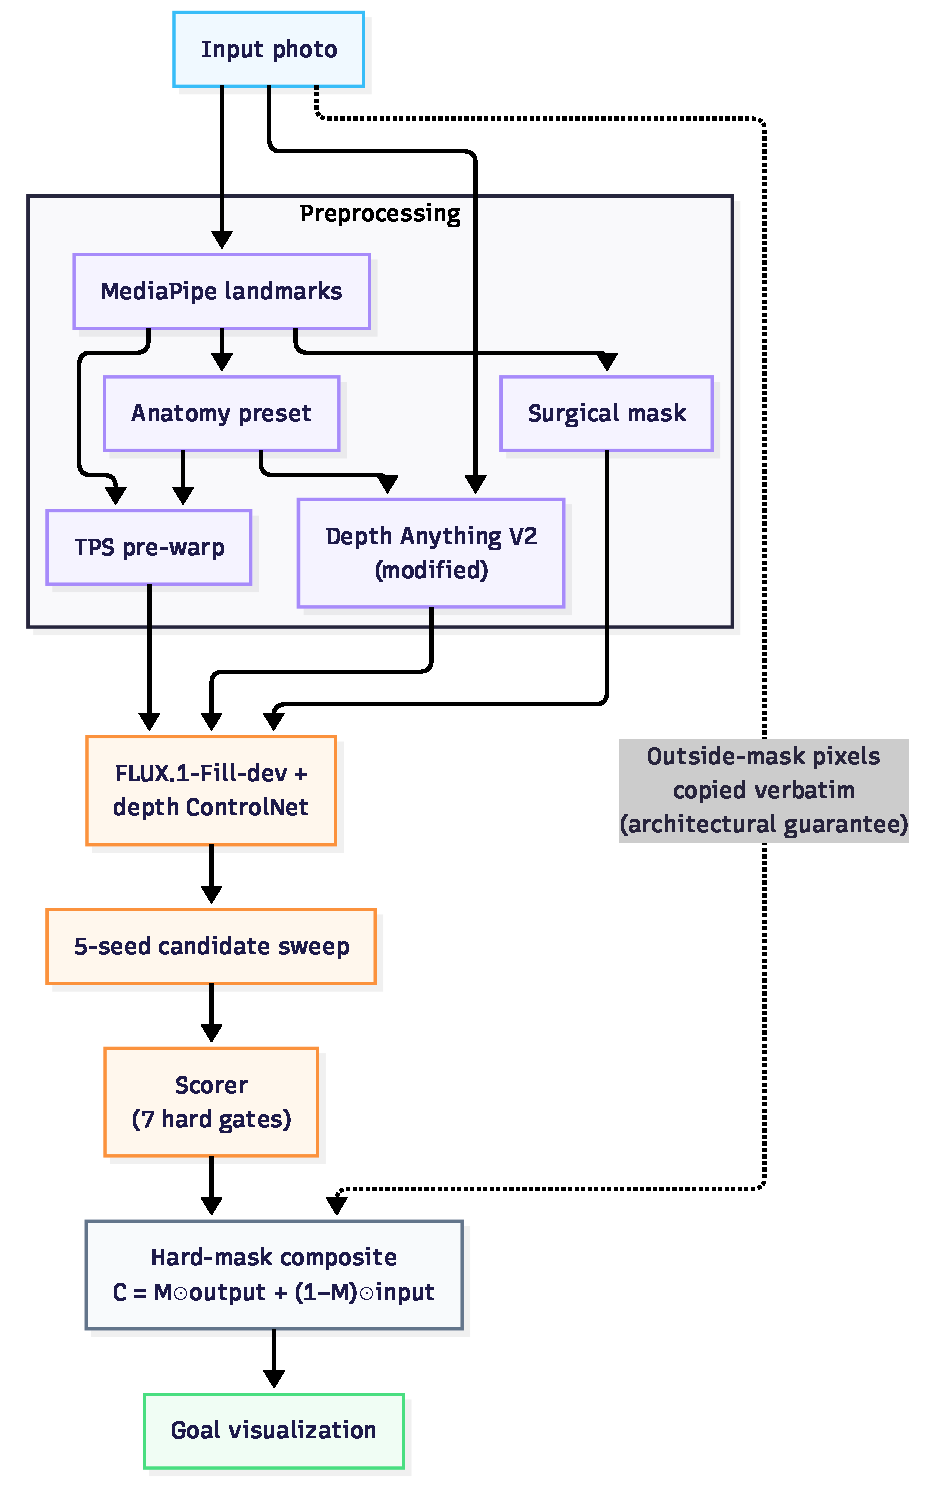
\includegraphics[width=0.55\linewidth]{figures/fig1_pipeline.pdf}
  \caption{\textbf{Envisage pipeline overview.}
    A preoperative photograph is processed in three stages: (1)~a
    procedure-specific TPS pre-warp displaces nasal landmarks by 2--4~px;
    (2)~Depth Anything~V2 estimates a monocular depth map, which is then
    modified by landmark-indexed Gaussian kernels to encode the intended tissue
    displacement; and (3)~FLUX.1-Fill-dev, conditioned on the modified depth
    map via a pretrained depth ControlNet, regenerates only the masked surgical
    region across a 5-seed candidate sweep. A 7-gate scorer selects the winning
    candidate, and a hard-mask composite pastes all non-surgical pixels verbatim
    from the input, so outside-mask identity preservation is architectural
    rather than a backbone property. We use the \emph{goal visualization}
    framing throughout, not patient-specific outcome prediction.}
  \label{fig:pipeline}
\end{figure}

\subsection{Mask Generation}

For rhinoplasty, 30 MediaPipe FaceLandmarker landmarks (478-point successor of the 468-vertex face mesh~\citep{kartynnik2019mediapipe}) spanning
the nasal dorsum, tip, and alar wings define the convex-hull mask, dilated
25 pixels with an elliptical structuring element and Gaussian-feathered
($\sigma{=}15$ pixels). The preset system (Section~\ref{sec:presets}) supports
8 frontal-detectable rhinoplasty sub-procedures whose masks extend the nasal core
to include the alar base, bridge sidewalls, and supratip region as needed.
The blepharoplasty mask spans 44 upper-lid and brow landmarks; the
rhytidectomy mask spans 36 jaw-contour landmarks. Both follow the same
dilation and Gaussian-feathering protocol as the rhinoplasty mask. Their
preset definitions are released as part of the framework but are not
the primary evaluation target of this paper.

\subsection{TPS Pre-Warp}

For rhinoplasty, bridge sidewall landmarks (indices 193, 245, 188, 174, 217 and
their right-side mirrors) are displaced inward by 3--4 pixels, tip lobule
landmarks inward by 2--3 pixels, and alar landmarks fixed at zero displacement.
The TPS uses \texttt{scipy.interpolate.RBFInterpolator} with a thin-plate
spline kernel and boundary anchor points to prevent deformation outside the
surgical region.

\subsection{Depth Modification}

Monocular depth was estimated with Depth Anything V2 Small~\citep{yang2024depth},
producing $D \in \mathbb{R}^{H \times W}$ normalized to $[0,255]$. Modified
depth is:
\begin{equation}
D'(x,y) = M(x,y) \cdot \bigl[D(x,y) - \textstyle\sum_k \alpha_k \cdot
G_k(x,y; c_k, \sigma_k)\bigr]
+ \bigl[1 - M(x,y)\bigr] \cdot D(x,y),
\label{eq:depth_mod}
\end{equation}
where $M$ denotes the binarized surgical mask used for depth modification (the feathered image-composite mask is a separate, image-domain quantity),
each $G_k$ is a 2D Gaussian at a landmark, and $\alpha_k$ controls
displacement magnitude. For rhinoplasty, two Gaussians are applied: a broad
one at the nasion (landmark~6, $\sigma_x{=}0.05w$, $\sigma_y{=}0.10h$,
$\alpha{=}100$) for dorsal hump reduction, and a tight one at the nasal tip
(landmark~1, $\sigma_x{=}0.015w$, $\sigma_y{=}0.15h$, $\alpha{=}115$) for
the supratip break. Amplitudes $\alpha_k$ are landmark-indexed hand-tuned constants
calibrated once on a held-out HDA case and held fixed for all reported evaluation runs;
evaluation uses 50\% default scaling, applied uniformly without per-cohort retuning. Depth modification does not distinguish
bony from cartilaginous deformation or model surgeon-specific choices such
as spreader-graft placement~\citep{daniel2010mastering}.

\subsection{Anatomy-Aware Preset System}
\label{sec:presets}

We encoded 8 of the 75 atomic rhinoplasty sub-procedures from Daniel's
\emph{Mastering Rhinoplasty} taxonomy~\citep{daniel2010mastering} that are
detectable from a single frontal photograph: dorsal hump reduction, tip
narrowing, bridge narrowing, alar base narrowing, dorsal straightening,
tip definition, tip rotation up, and nose shortening. Each sub-procedure has a landmark-measurement detection threshold
and a prompt fragment. The prompt builder selects the top 3 detected
sub-procedures by a fixed clinical-priority ordering (PRIORITY\_ORDER in \texttt{rhino\_config.py}, derived from Daniel's taxonomy frequency rankings) and concatenates their fragments,
producing a subject-specific prompt. The blepharoplasty (8) and
rhytidectomy (8) preset definitions follow the same architecture using
Tessier orbital and SMAS-layer anatomy respectively; they are released as part of the
framework.

\subsection{Diffusion Inpainting}

FLUX.1-Fill-dev~\citep{flux2024}, a 12-billion-parameter rectified flow fill model, is
used with a pretrained depth ControlNet~\citep{zhang2023controlnet}
(\texttt{jasperai/Flux.1-dev-Controlnet-Depth}) at conditioning scale 0.5.
The \texttt{FluxInpaintPipeline} uses guidance scale 3.5, 20 denoising steps,
BF16 precision, and $512 \times 512$ resolution. Inpainting strength for
rhinoplasty is 0.75 at 50\% depth modification intensity. No procedure-specific
training is required for the base pipeline (a separate DPO LoRA probe is reported in Appendix~\ref{app:dpo_hparams}).

\subsection{Mask-Decomposed Evaluation: SurgicalScore}
\label{sec:eval_metric}

Standard full-face metrics conflate two distinct objectives: outside-mask
fidelity to the input, and inside-mask accuracy against the ground-truth
postoperative image. We define \textbf{SurgicalScore}, which decomposes
evaluation by mask region and reference:
\begin{itemize}
\item \textbf{Outside-mask SSIM}: prediction vs.\ input on pixels where
  $M < 0.5$. Approaches 1.0 for methods preserving non-surgical regions.
\item \textbf{Inside-mask LPIPS}: prediction vs.\ ground truth on the mask
  bounding crop (AlexNet backbone~\citep{zhang2018lpips}).
\item \textbf{Input ArcFace}: output vs.\ input cosine similarity (identity
  preservation).
\item \textbf{GT ArcFace}: output vs.\ ground truth cosine similarity (postoperative target-proximity proxy in identity space).
\item \textbf{BL ArcFace}: input vs.\ ground truth (dataset-level baseline,
  not a method score).
\end{itemize}

Because the composite $C = M \odot G + (1-M) \odot I$ differs from the input
only on the masked region, the operational identity preservation reduces to
the directly measurable outside-mask SSIM, which exceeds $0.999$ across all
evaluated cohorts (a property of the compositing rule, not of any backbone).
Empirically, the local Lipschitz constant of ArcFace under masked perturbations
is bounded by $L_{p95} \leq 1.2 \times 10^{-5}$ ($N{=}255$ samples,
Appendix~\ref{app:sensitivity}).

A \textbf{Mask-Area Modifier} corrects small-mask inflation: metrics are computed
on a resize-to-256 crop of the mask bounding box to normalize the effective
contribution of the surgical region. The affine rescale (slope 0.70, intercept 0.30) anchors the
passthrough floor at 0.30, so any SurgicalScore below 0.30 is scored below
returning the input under the protocol. Component weights are protocol hyperparameters; the floor is set by the affine rescale, not by the weights.

This decomposition prevents the confound observed in prior work~\citep{landmarkdiff_anon},
where over 95\% of the identity score originated from composited pixels
(0.509 composited vs.\ 0.023 without).

\paragraph{SurgicalScore composite.}
For scored validation cases, the five components are aggregated as:
\begin{equation}
\mathrm{SS} = 0.30 + 0.70 \cdot \frac{R_O - R_I}{1 - R_I}, \quad
R_O = 0.40\,A + 0.30\,B + 0.15\,C + 0.10\,D + 0.05\,E
\label{eq:ssv5}
\end{equation}
where $R_I$ is $R_O$ evaluated with $O = I$ (the passthrough reference),
and a hard ArcFace identity gate disqualifies candidates when
$\cos(I, O) < 0.65$ (Input ArcFace, input-to-output). Component weights balance directional
and fidelity terms; the passthrough floor at $0.30$ is set by the affine rescale (slope $0.70$,
intercept $0.30$). Both are protocol hyperparameters fixed before any cross-method comparison.
SurgicalScore is the diagnostic protocol; cross-method ranking uses the GT-vs-BL ArcFace gap,
an independent embedding metric.
The five components: $A$ = directional alignment (cosine of morphometry edit vectors,
as in~\citet{gal2022stylegan_nada}); $B$ = edit magnitude fit (asymmetric log-ratio,
over-edit penalized at $1.5\times$, under-edit at $1.0\times$); $C$ = masked LPIPS
fidelity on a 256$\times$256 mask-crop resize (Mask-Area Modifier applied); $D$ =
face realism: mean of SER-FIQ~\citep{terhorst2020serfiq} and CR-FIQA~\citep{boutros2023crfiqa} quality scores, with a three-signal proxy (embedding norm, Laplacian variance, color balance) as fallback when FIQA models are unavailable; $E$ = outside-mask
soft preservation ($1 - \mathrm{LPIPS}_\text{out} / \tau$, $\tau{=}0.10$).
\citet{gal2022stylegan_nada} introduced directional cosine loss in image editing;
$A$ adapts this to procedure morphometry space.
The rhinoplasty morphometry vector $\phi_\text{morph}^\text{rhino} \in \mathbb{R}^5$ contains:
Goode ratio~\citep{goode1984rhinoplasty} (lateral-view approximation computed from frontal photographs: tip projection / nasal length);
nasolabial angle (lateral-view approximation computed from frontal photographs, subnasale, landmark 2); alar width / intercanthal distance;
dorsal line RMS deviation / nasal length; nasal length / face height.
All components are scale-invariant ratios or normalized angles.

\paragraph{SS\textsubscript{raw} calibration anchor.}
SurgicalScore is the calibrated metric used for all cross-method comparison.
The uncalibrated raw composite $R_O = 0.40\,A + 0.30\,B + 0.15\,C + 0.10\,D + 0.05\,E$
(without the passthrough-anchored affine rescale) is reported alongside as a calibration
check; we refer to it as SS\textsubscript{raw}.
Under SS\textsubscript{raw}, an oracle control in which the system output is replaced
directly by the ground-truth postoperative image (no hard-mask composite) achieves
$0.919$ $[0.918, 0.920]$ on the $N{=}211$ cohort ($B{=}10{,}000$ bootstrap).
This confirms the metric ceiling is achievable for a perfect predictor and that the
score range $[0,\,1]$ is used as intended.
Aggregate \method{} SS\textsubscript{raw} on $N{=}211$ is $0.563$ $[0.536, 0.590]$.
SS\textsubscript{raw} values for all ablation variants appear in
Table~\ref{tab:composite_ablation}.

\paragraph{Component-level discrimination.}
Each of the five SurgicalScore components flags failures the others miss.
Case Nose\_33 receives outside-mask preservation score ($E$) $= 0.000$ from a
compositing artifact in the mask boundary region despite high directional alignment
($A = 0.997$) and edit magnitude ($B = 0.872$), traced to
\texttt{evaluation/surgicalscore\_v5\_fixed\_hda\_rhino.json}.
Case Nose\_154 receives directional alignment ($A$) $= 0.004$ from a preset selection
mismatch despite intact realism ($D = 0.738$) and outside-mask preservation
($E = 0.540$).
Case Nose\_161 receives edit magnitude ($B$) $= 0.049$ from insufficient in-mask change
despite high directional alignment ($A = 1.000$) and realism ($D = 0.736$).
These three cases are not discriminable on full-face ArcFace alone: their
$\cos(\text{input}, \text{output})$ scores are 0.740, 0.858, and 0.692,
respectively, all above the identity gate threshold.

\subsection{Decision Model}
\label{sec:decision_model}

Seven hard gates must be passed for a candidate to be valid: (1) identity:
Input ArcFace $\geq 0.65$; (2) outside-SSIM: $\geq 0.95$; (3) landmark
drift: $\leq 15.0$ px; (4) dark-hole: mask HSV-V$<$20 area $\leq 0.5\%$;
(5) color consistency: mean hue shift $\leq 15.0^\circ$; (6) crease: blepharoplasty only;
(7) procedure fidelity: landmark-atlas severity bands. Passing candidates are
ranked by a weighted composite (0.25 identity, 0.15 outside-SSIM, 0.15
landmark drift, 0.15 color consistency, 0.15 cross-method agreement, 0.10 TPS agreement,
0.05 aesthetic). Cross-method agreement is computed only among \method{}'s own
candidate seeds and the deterministic TPS/preset proxies; no baseline outputs
or postoperative ground truth are used for candidate selection. If no
diffusion candidate passes, the deterministic TPS warp ($M5$) is substituted
as a non-generative geometric fallback.

%% ========================================================================
%% 4. EXPERIMENTS
%% ========================================================================
\section{Experiments}
\label{sec:experiments}

\subsection{Dataset}

We use two cohorts: HDA~\citep{rathgeb2020plastic} for matched paired
pre/post photographs across procedures, and an external ASPS+PCA
rhinoplasty cohort for the headline comparison. The HDA Plastic Surgery
Database contains 638
subjects. The matched HDA test splits contain 27 blepharoplasty, 21 rhinoplasty,
and 9 rhytidectomy pairs. The headline rhinoplasty comparison
(Section~\ref{sec:results}, Table~\ref{tab:strict_n211}) uses the
$N{=}211$ ASPS/PCA cohort described below. The matched 21-pair HDA
rhinoplasty split is used for the DPO pilot probe (Appendix~\ref{app:dpo_hparams})
and for prior-work comparability in Appendix~\ref{app:n21_detailed}.

We further assembled an external validation corpus from ASPS Photo
Gallery~\citep{asps2024gallery} and an additional private clinical archive
of paired pre/post photographs (\emph{PCA}), filtered to frontal views
(InsightFace yaw-symmetry $\geq 0.82$) and pre/post identity floor
($\geq 0.35$ ArcFace cosine), yielding 457 rhinoplasty pairs. All external
pairs are held out from training, hyperparameter selection, and preset design.

HDA is the only public corpus with identity-paired pre/post photographs across
the three procedures; CelebA-HQ~\citep{karras2018celebahq} and
FFHQ~\citep{karras2019ffhq} contain none, commercial 3D platforms are
proprietary, and SurFace1259~\citep{varghaei2025surface} was unavailable.
The identity-floor filter excludes pairs whose appearance change exceeds
plausible surgical drift; \texttt{rhytidectomy\_Facelift\_08} is removed
after manual review identified two different subjects.

\subsection{Baselines}

Three instruction-conditioned baselines were evaluated under two protocols: the $N{=}211$ ASPS+PCA cohort (used for the headline comparison in Table~\ref{tab:strict_n211}) and the matched $N{=}21$ HDA paired pool (used for prior-work comparability in Appendix~\ref{app:n21_detailed}): (1)~\textbf{InstructPix2Pix}~\citep{brooks2023instructpix2pix},
a full-image text-instruction editor applied with the same preset-derived
prompts; (2)~\textbf{ICEdit}~\citep{zhang2025icedit}, FLUX.1-Fill-dev with a
MoE-LoRA via diptych inference; (3)~\textbf{FLUX.1-Kontext-dev}~\citep{flux_kontext_2025},
a text-conditioned image-to-image variant run zero-shot followed by the same
hard-mask composite used in \method{}.

Three internal diagnostic baselines accompany the main comparators: Direct Copy
(Input ArcFace $=1.0$ upper bound), TPS Warp (geometric morphing only), and
FLUX Inpainting without ControlNet.

\subsection{Implementation}

Inference runs on a single NVIDIA L40S GPU (48~GB) in BF16. Depth estimation
uses Depth Anything V2 Small~\citep{yang2024depth}. Landmarks use MediaPipe FaceLandmarker
(478 points; successor of the 468-vertex face mesh~\citep{kartynnik2019mediapipe}). ArcFace uses InsightFace buffalo\_l
(R50). LPIPS uses AlexNet~\citep{zhang2018lpips}. Inference takes approximately
20 seconds per image. Training details for the DPO LoRA are given in
Appendix~\ref{app:dpo_hparams}.

\subsection{Statistical Inference}

We computed 95\% confidence intervals (CIs) on reported means wherever per-case
or seed-level replicates were available, via percentile bootstrap ($B{=}10{,}000$
resamples, seed~42). For Table~\ref{tab:surgical_score}
\method{} rows, matched-$N$ per-case GT Arc scores were not available locally;
CIs were bootstrapped over five seed-level means (denoted $\dagger$). ICEdit
CIs were bootstrapped over per-case scores ($N{=}21$). IP2P and Kontext
per-case data were not available; their CIs are not reported.

Bootstrapping over seed-level means captures inference variance (sensitivity to
random initialization) but not case-level variance (sensitivity to which 21
cases constitute the test set). The reported $95\%$ CIs are therefore not estimates
of case-sampling uncertainty: they reflect seed-to-seed reproducibility, not
the full uncertainty that would be estimated from a larger rhinoplasty population.

Within-protocol Input ArcFace ordering: \method{} exceeded ICEdit on rhinoplasty
($p{=}0.0361$, $N_{\text{ours}}{=}16$, $N_{\text{ice}}{=}21$, two-sample 10,000-permutation, two-sided).
This test is included for protocol consistency; cross-method ordering on Input ArcFace is
not informative of inside-mask quality, since the metric is structurally confounded by
hard-mask compositing. For the $N{=}211$ cohort, paired sign-flip permutation tests against each
baseline are reported in Table~\ref{tab:paired_n205} ($p < 10^{-4}$ all three).
For the matched $N{=}21$ DPO probe, per-case zero-shot GT ArcFace was not stored
at evaluation time, so the probe is directional only.

%% ========================================================================
%% 5. RESULTS
%% ========================================================================
\section{Results}
\label{sec:results}

\paragraph{Cohorts.} External corpus assembly: 457 raw rhinoplasty pairs from
ASPS Photo Gallery ($N{=}441$) and PCA ($N{=}16$). Two filtered cohorts derive
from this pool: (a) the $N{=}211$ cohort (ASPS $=202$, PCA $=9$)
requires both MediaPipe landmark detection and pre/post ArcFace $\geq 0.65$;
this is the headline cohort. (b) The gate-pass $N{=}438$ subset
(ASPS $=422$, PCA $=16$) requires only ArcFace $\geq 0.65$ on at least one
of five seeds; reported as the external gate-pass rate in
Section~\ref{sec:surgeon-verification} and the source-stratified pooled
GT-vs-BL replication in Appendix~\ref{app:external_sources}. (c) Matched $N{=}21$ HDA rhinoplasty
pool, used for the DPO probe and Appendix~\ref{app:n21_detailed}.

\subsection{Headline ArcFace and SurgicalScore on Rhinoplasty}

\paragraph{ArcFace headline.}
Table~\ref{tab:strict_n211} gives the headline result on the $N{=}211$
rhinoplasty cohort: ASPS public gallery ($N{=}202$) and a private clinical
archive (PCA, $N{=}9$), filtered to cases passing MediaPipe landmark
detection and pre/post same-person ArcFace at $0.65$ cosine. Across all
four methods evaluated, no method achieves positive mean GT ArcFace gain
over the unedited preoperative input. \method{} achieves output-to-GT
cosine $0.662$ versus input-to-GT $0.711$, gap $-0.048$ ($95\%$ CI
$[-0.055, -0.042]$, $B{=}10{,}000$); ICEdit, Kontext, and IP2P gaps are
$-0.139$, $-0.242$, $-0.294$ with non-overlapping CIs
(Table~\ref{tab:strict_n211}). On the four-way detected intersection
($N{=}205$), \method{} reduces the gap by $+0.090$ vs.\ ICEdit, $+0.189$
vs.\ Kontext, and $+0.245$ vs.\ IP2P, all paired sign-flip permutation
$p < 10^{-4}$ (Table~\ref{tab:paired_n205}). The fraction of cases where
output exceeds input proxy under GT ArcFace is $16.1\%$ for \method{}
versus $0.0$/$4.3$/$1.0\%$ for the baselines.

\paragraph{SurgicalScore.}
Mean SurgicalScore on \method{} on this cohort is $0.599$ $[0.579, 0.619]$
vs.\ ICEdit $0.502$ $[0.467, 0.535]$, InstructPix2Pix $0.337$
$[0.295, 0.380]$, and FLUX.1-Kontext-dev $0.229$ $[0.188, 0.271]$
(Appendix~\ref{app:ss_strict}, Table~\ref{tab:ss_strict_n211}). On the
four-way detected intersection ($N{=}188$), \method{} exceeds ICEdit by
$\Delta{=}+0.091$, InstructPix2Pix by $\Delta{=}+0.264$, and Kontext by
$\Delta{=}+0.368$, all paired sign-flip permutation $p < 10^{-4}$. $98.6\%$
of cases clear $0.35$ and $68.7\%$ clear $0.50$.

\paragraph{Operational.}
The pipeline verdict is \textsc{pass} on $208/211$ and \textsc{borderline}
on $3/211$. The TPS fallback (M5) was not substituted on any $N{=}211$
case ($0/211$); fallback fired on $3/57$ ($5.3\%$) of the matched HDA
pool. The $N{=}457$ external corpus passes the identity gate at $95.8\%$
($438/457$).

Outside-mask SSIM exceeds $0.999$ for \method{} by architectural
construction; the same property holds for Kontext under the same composite
(Appendix~\ref{app:composite_full}), confirming the preservation follows
from the compositing rule, not from any one backbone. Mask-crop LPIPS
replicates the ranking: \method{} matches input-proxy LPIPS within
$\pm 0.012$, while baselines drift $0.12$--$0.20$ further from GT
(Appendix~\ref{app:mask_crop}). The methodological diagnosis transfers
across procedures (Appendix~\ref{app:cross_proc}).

\begin{table}[t]
\centering
\small
\caption{\textbf{Main result on the $N{=}211$ rhinoplasty cohort}
(ASPS public gallery $N{=}202$ + PCA private clinical archive $N{=}9$,
passing MediaPipe landmark detection and same-person ArcFace at $0.65$
cosine). \textbf{No method achieves positive mean GT ArcFace gain over the
unedited preoperative input.} \method{} achieves the smallest gap of any
method evaluated, with $16.1\%$ of cases positive ($0.0$/$4.3$/$1.0\%$ for
ICEdit/Kontext/IP2P). Per-method $N$ varies
due to InsightFace detection failures on a subset of generated outputs;
BL Arc is computed on the corresponding per-method input subset, so each
method's gap is paired within its own attrition mask. Gap 95\% CIs are
percentile bootstrap over per-case scores ($B{=}10{,}000$, seed~42).
\%~Pos.\ is the fraction of cases where output-to-GT ArcFace exceeds
input-to-GT ArcFace; \method{} is the only method exceeding $5\%$.
Paired statistical comparisons against \method{} are reported in
Table~\ref{tab:paired_n205}.}
\label{tab:strict_n211}
\begin{tabular}{@{}lccccc@{}}
\toprule
\textbf{Method} & \textbf{N} & \textbf{GT Arc}$\uparrow$ & \textbf{BL Arc} & \textbf{Gap [95\% CI]} & \textbf{\% Pos.}$\uparrow$ \\
\midrule
InstructPix2Pix     & 208 & 0.417 & 0.711 & $-0.294$~$[-0.331, -0.256]$ & 1.0 \\
ICEdit              & 206 & 0.573 & 0.712 & $-0.139$~$[-0.148, -0.130]$ & 0.0 \\
FLUX.1-Kontext-dev  & 211 & 0.469 & 0.711 & $-0.242$~$[-0.258, -0.225]$ & 4.3 \\
\method{} (ours)    & 211 & \best{0.662} & 0.711 & \best{$-0.048$~$[-0.055, -0.042]$} & \best{16.1} \\
\bottomrule
\end{tabular}
\end{table}

\begin{table}[t]
\centering
\small
\caption{\textbf{Paired comparison against \method{} on the four-way detected
intersection ($N{=}205$).} Each baseline is restricted to the cases where all
four methods produced a detected face, and the per-case ArcFace gap (output-to-GT
minus input-to-GT) is differenced row-wise against \method{}. Positive $\Delta$
favors \method{}. CI is percentile bootstrap over per-case differences
($B{=}10{,}000$). $p$ is a paired sign-flip permutation test
($B{=}10{,}000$). All three baselines are rejected against \method{} at
$p < 10^{-4}$.}
\label{tab:paired_n205}
\begin{tabular}{@{}lccc@{}}
\toprule
\textbf{Comparison (\method{} $-$ X)} & \textbf{$\Delta$ Gap} & \textbf{95\% CI} & \textbf{$p$ (paired perm.)} \\
\midrule
\method{} $-$ ICEdit            & $+0.090$ & $[+0.079, +0.101]$ & $<10^{-4}$ \\
\method{} $-$ FLUX.1-Kontext-dev & $+0.189$ & $[+0.172, +0.205]$ & $<10^{-4}$ \\
\method{} $-$ InstructPix2Pix    & $+0.245$ & $[+0.207, +0.285]$ & $<10^{-4}$ \\
\bottomrule
\end{tabular}
\end{table}

% Legacy N=21 detailed table moved to Appendix~\ref{app:n21_detailed}
% to fit NeurIPS 9-page main paper limit. Headline N=211 numbers
% are reported in Table~\ref{tab:strict_n211} above.

% Figure: SurgicalScore decomposition moved to Appendix~\ref{app:decomposed_fig}.

% §5.2 DPO LoRA Pilot Probe and the N=211 six-configuration $\beta$-sweep
% are reported in Appendix~\ref{app:dpo_hparams} and Appendix~\ref{app:dpo_sweep};
% both are negative results retained for transparency and are not part of the
% paper's main claim.

\paragraph{External cohort and surgeon review.}\label{sec:surgeon-verification}
On the $457$-pair external corpus, pooled GT Arc $0.597$ vs.\ BL Arc
$0.664$ (gap $-0.067$ vs.\ $-0.048$ on $N{=}211$, Appendix~\ref{app:external_sources}):
the negative gap holds on the broader cohort, larger magnitude consistent
with more difficult cases. A board-certified surgeon judged six outputs
plausible while flagging over-symmetrization; multi-rater blinded GAIS/ROE
is future work.

\paragraph{Discussion and limitations.}\label{sec:discussion}\label{sec:conclusion}\label{sec:limitations}
\method{} is a pre-consult goal-visualization tool and evaluation protocol,
not a patient-specific outcome predictor. Headline claims are
rhinoplasty-specific; blepharoplasty and rhytidectomy preset definitions
are released as framework infrastructure with cross-procedure results in
Appendix~\ref{app:cross_proc}. The negative ArcFace gap across all
evaluated methods establishes that full-face identity verification cannot
grade localized surgical edits, the paper's central diagnostic claim.
Per-case oracle selection over five seeds reduces the residual gap by
$73\%$ to $-0.015$ with $33.9\%$ of cases positive
(Appendix~\ref{app:best_of_k}), indicating substantial candidate-space
headroom; the open problem is a deployable non-oracle ranker
(Appendix~\ref{app:deployable_ranker}, full limitations
Appendix~\ref{app:limitations_full}).



%% ========================================================================
%% REFERENCES
%% ========================================================================
\bibliographystyle{plainnat}
\bibliography{refs}

%% ========================================================================
%% APPENDIX
%% ========================================================================
\appendix

\section{Deployable K$=5$ Ranker Probe}
\label{app:deployable_ranker}

The K$=5$ best-of-$5$ oracle assumes GT access at scoring time. To assess
whether a deployable (no-GT) ranker can recover the oracle gain, we
evaluated six GT-free per-seed signals as candidate rankers on the
five-seed-complete subset ($N{=}207$): random selection, single fixed seed
(K$=1$ headline), max ArcFace$(out, in)$ (identity preservation), max
realism component~D, ArcFace$\times$D, and max outside-mask SSIM.
None recovered any of the K$=1{\rightarrow}$K$=5$ oracle gain
($+0.134$); all underperformed K$=1$ by $0.01$--$0.04$. Detail in
Table~\ref{tab:deployable_ranker}.

\begin{table}[h]
\centering
\small
\caption{Naive no-GT rankers vs.\ K$=5$ oracle on $N{=}207$ (Envisage
five-seed-complete cases). Per-case oracle selection by true SurgicalScore
raises the mean from $0.609$ (K$=1$) to $0.743$ ($+0.134$). Deployable
rankers based on identity preservation ($\arccos(O,I)$), realism (D),
outside-mask SSIM (E), or combinations all score below the single-seed
headline; the oracle gain comes from GT-aware components (A directional,
B magnitude, C masked LPIPS) that no-GT signals do not approximate.
A learned non-oracle ranker trained on (image, predicted SurgicalScore)
pairs is the natural next step; this is future work.}
\label{tab:deployable_ranker}
\begin{tabular}{@{}lcc@{}}
\toprule
\textbf{Ranker} & \textbf{Mean SS} & \textbf{$\Delta$ vs.\ K$=1$} \\
\midrule
Random seed                         & $0.574$ & $-0.035$ \\
\textbf{K$=1$ (seed $42$, headline)} & $\mathbf{0.609}$ & $0.000$ \\
$\arccos(O,I)$ (identity preservation) & $0.597$ & $-0.012$ \\
D (realism)                         & $0.580$ & $-0.029$ \\
$\arccos(O,I) \cdot D$              & $0.600$ & $-0.009$ \\
E (outside-mask SSIM)               & $0.595$ & $-0.014$ \\
\midrule
K$=5$ oracle (max true SS)          & $\mathbf{0.743}$ & $\mathbf{+0.134}$ \\
\bottomrule
\end{tabular}
\end{table}

\paragraph{Per-ranker interpretation.}
Each ranker's failure mode reflects a specific GT-blind tradeoff.
$\arccos(O,I)$ maximizes input--output similarity, which selects for
\emph{minimal} edit, the opposite of what the metric rewards (directional
alignment $A$ and magnitude $B$). $D$ (realism via FIQA) rewards
photorealistic outputs but does not correlate with surgical correctness; a
high-realism candidate may edit in the wrong direction.
$\arccos(O,I) \cdot D$ combines two GT-blind signals without resolving the
underlying GT-blindness. $E$ (outside-mask SSIM) is nearly identical
across seeds because the composite preserves outside-mask pixels by
construction, so the signal carries almost no per-seed information. Random
selection underperforms by construction. The common failure mode: GT-aware
components ($A$ directional, $B$ magnitude, $C$ masked LPIPS) drive the
$+0.134$ oracle gain, and no GT-free signal approximates them.

\paragraph{Learned-ranker sketch.}
A learned non-oracle ranker
$f(I_{\text{candidate}}, I_{\text{input}}, \ell_{\text{edit}}) \to \widehat{SS}$
predicting SurgicalScore from image and landmark features could
potentially recover the oracle gain at deployment. Training data already
exists: the $5$-seed $\times$ $N{=}211$ sweep yields $1{,}055$
(candidate, SurgicalScore) pairs, sufficient for fitting a small
regression head on pretrained features (e.g., DINOv2~\citep{oquab2024dinov2}
$+$ MLP, or a fine-tuned ViT). Held-out $N{=}21$ HDA matched cases provide
independent validation. The architectural separation between substrate
(this paper) and ranker (future work) means a successful ranker is a pure
post-hoc improvement: it does not require retraining the diffusion
backbone, and the current pipeline's K$=1$ outputs serve as the floor any
deployable ranker must clear. Open question: whether the (image, predicted
$SS$) supervision signal is dense enough to learn the GT-aware components
implicit in $A$, $B$, and $C$, or whether ranker training requires
additional clinical labeling.

\section{Detailed Limitations}
\label{app:limitations_full}

\textit{Statistics.} $N{=}211$ uses per-case bootstrap and paired
permutation; matched $N{=}21$ DPO probe is directional only because
zero-shot per-case GT ArcFace was not stored.

\textit{Clinical evaluation depth.} Aesthetic plausibility was assessed by
a single board-certified facial plastic surgeon coauthor on six
representative outputs. This is a feasibility check, not a clinical study.
A multi-rater blinded panel evaluation using validated instruments (GAIS,
ROE) on a larger output sample is committed pre-deployment work.

\textit{2D representation constraints.} The pipeline operates on a single
frontal photograph and a 2D monocular depth map. This representation
cannot disambiguate bony vs.\ cartilaginous nasal deformation, model
surgeon-specific structural choices (e.g., spreader-graft placement,
septal reconstruction), or render lateral or oblique views. The qualitative failure mode of rhinoplasty volumetric miss reflects
this constraint: cases requiring full 3D shape change exceed what 2D
depth conditioning can encode.

\textit{Consent and governance.} HDA is used under its biometric-research
license; ASPS public-gallery and PCA clinical-archive images are used for
held-out evaluation only without redistribution. Released artifacts are
code, evaluation harnesses, preset configurations, and split manifests.
Clinical deployment beyond goal-visualization scope requires multi-site
IRB review.

\textit{Anchoring risk.} Photorealistic outcome visualizations can anchor
patient expectations regardless of framing; the symmetry bias the surgeon
identified is one manifestation. Clinical deployment must pair the
visualization with explicit verbal anchoring during counseling.

\textit{Ranker design and appearance norms.} The K$=5$ oracle result
implies that future work will design a non-oracle candidate ranker. A
ranker trained on aesthetic preferences, surgeon ratings, or any reward
signal that encodes appearance norms would risk filtering candidates
toward an idealized phenotype rather than the patient-specific surgical
outcome. Ranker design must explicitly address this risk: audit ranker
preferences for race, gender, age bias; require multiple suggestions
surfaced rather than a single recommended one.

\textit{Fairness power analysis.} The Monk Skin Tone stratification
reports $N{=}4$ on tone~$7$, which is too small for a powered claim.
Under $\alpha{=}0.05$ and a two-sided test for a SurgicalScore difference
of $0.05$ against the N=211 variance, characterizing the gap with
$80\%$ power requires $N{=}25$--$40$ per stratum on tones $7$--$10$;
recruiting that cohort is committed pre-deployment work.

\section{ArcFace as Identity Gate, Not Surgical-Fidelity Metric}
\label{app:arcface_gate}

ArcFace is trained for full-face verification and compresses the entire
face into a $512$-d embedding dominated by stable features (eye geometry,
jawline curvature, skull shape, hairline). The embedding mixes a small
localized change with the much larger global identity signal, so changes
at the scale of surgical rhinoplasty (mean mask area $3.65\%$ of pixels
across the $N{=}211$ cohort, range $1.32$--$10.90\%$) produce signal that
the metric registers but cannot attribute to surgical correctness. The same postoperative target is identified
as the same person as the preoperative input at high cosine ($0.71$)
precisely because rhinoplasty preserves global identity. The $-0.048$
N=211 gap reflects two things: a small ArcFace noise floor under
any pixel-level perturbation of the face (consistent across all four
tested methods, see paired comparisons in Table~\ref{tab:paired_n205}),
and a small diffusion artifact in the inpainted region that the metric
notices without being able to attribute to whether the change is
surgically correct. Per-case oracle selection over five seeds reduces the
gap by $73\%$ to $-0.015$ and produces positive identity gain on $33.9\%$
of cases (Appendix~\ref{app:best_of_k}), which is the correct read of the
candidate-space ceiling under our pipeline. We retain ArcFace as a strict
identity gate (output must remain identifiable as the same person,
$\cos\!\geq\!0.65$), which it is well-suited for, but not as a primary
outcome metric, which it was never designed to be. SurgicalScore,
landmark-derived edit vectors, and masked LPIPS serve the
continuous outcome-grading role; the two roles are complementary, not
redundant.

\section{SurgicalScore Decomposition Figure}
\label{app:decomposed_fig}

\begin{figure}[h]
  \centering
  
\includegraphics[width=0.85\linewidth]{figures/fig3_decomposed_arcface}
  \caption{\textbf{Diagnostic comparison of full-face identity similarity and
    non-surgical-region preservation on the $N{=}211$ rhinoplasty
    cohort.}
    The non-surgical region is preserved by the hard-mask composite, so high
    full-face identity scores are dominated by copied pixels and should not be
    interpreted as surgical accuracy. This is a preservation diagnostic, not an
    additive decomposition of ArcFace (full-face ArcFace cosine is not
    region-additive). \method{} achieves output-to-GT ArcFace $0.662$ versus
    the input-to-GT proxy $0.711$ (gap $-0.048$); outside-mask SSIM is $1.000$
    by construction. The GT-below-BL gap is the central open problem, and
    SurgicalScore (Section~\ref{sec:eval_metric}) provides the mask-decomposed
    metric we use for cross-method comparison. Cross-procedure validation
    appears in Appendix~\ref{app:cross_proc}.}
  \label{fig:decomposed_arcface}
\end{figure}

\section{Qualitative Rhinoplasty Outputs}
\label{app:qualitative_fig}

\begin{figure}[h]
  \centering
  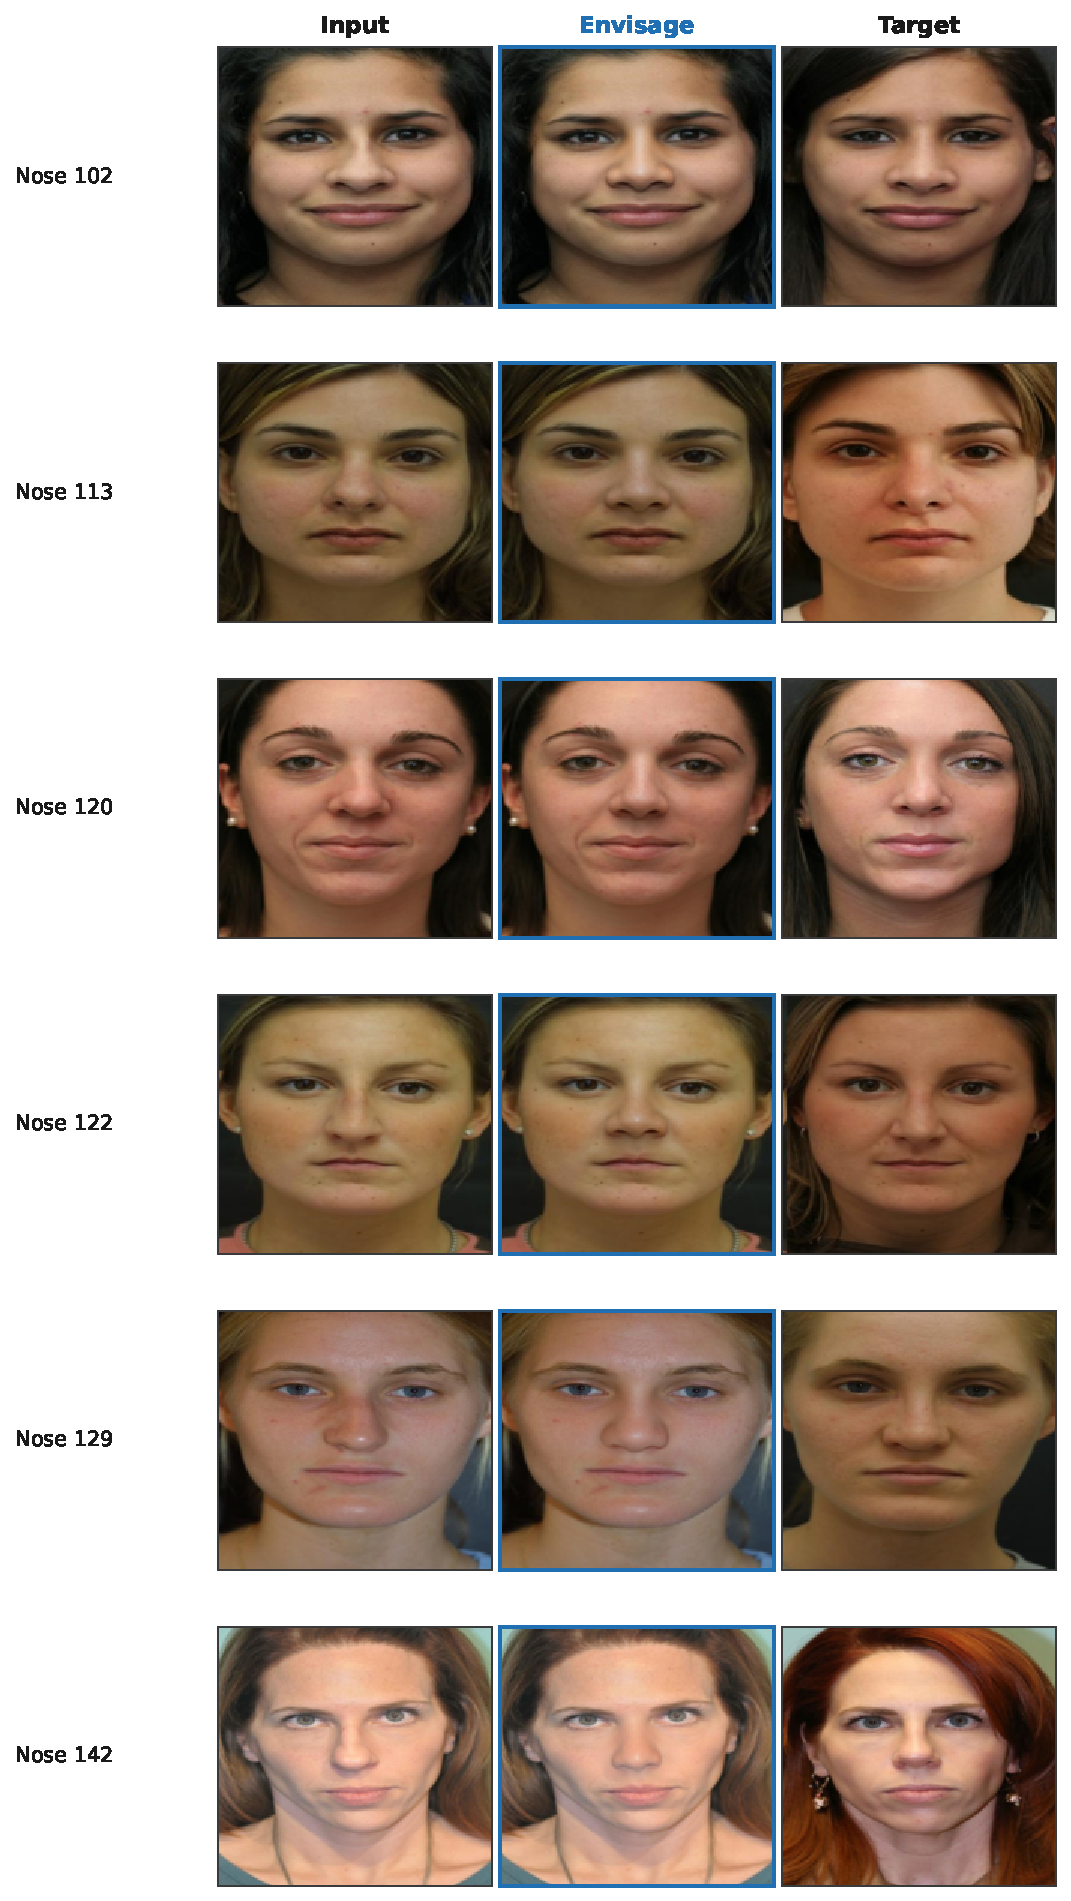
\includegraphics[width=0.65\linewidth,keepaspectratio]{figures/fig_qualitative_v26}
  \caption{\textbf{Six surgeon-reviewed rhinoplasty cases} (Nose\_102,
    113, 120, 122, 129, 142). Columns: input, \method{} prediction,
    postoperative target. The board-certified facial plastic surgeon
    coauthor judged each as a goal-setting visualization on the matched
    HDA pool. Inside the mask the pipeline produces anatomically
    plausible edits; outside the mask identity preservation is exact by
    construction. Nose\_120 illustrates the symmetry-bias caveat
    described in Section~\ref{sec:limitations}.}
  \label{fig:qualitative_rhinos}
\end{figure}

\begin{figure}[h]
  \centering
  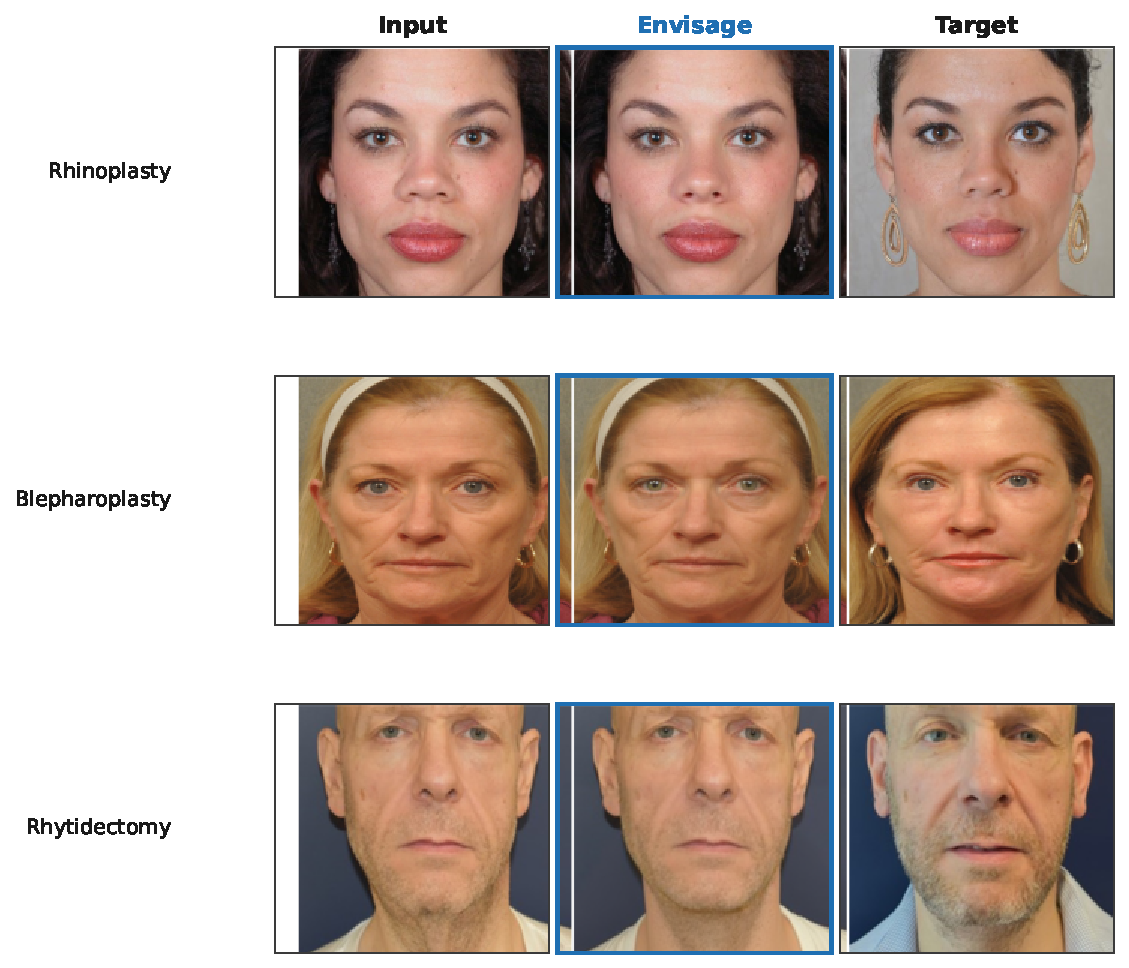
\includegraphics[width=0.85\linewidth,keepaspectratio]{figures/fig_other_procedures}
  \caption{\textbf{Cross-procedure preset visualization on three subjects
    (frontal view, intensity $=60$).} Five rows correspond to the
    non-rhinoplasty procedures covered by the released preset taxonomy
    (blepharoplasty, rhytidectomy, orthognathic, brow lift, mentoplasty);
    three column-pairs show before/after on three independent synthetic
    subjects. All cells are rendered from the identical frontal pose, so
    differences across rows reflect preset-level edits and differences
    across columns reflect subject anatomy. Source:
    \texttt{demos/procedure\_comparison\_all\_subjects.png} from the
    public release.}
  \label{fig:other_procedures}
\end{figure}

\section{Detailed N=21 Matched HDA Paired-Pool Metrics}
\label{app:n21_detailed}

On the matched $N{=}21$ HDA rhinoplasty paired pool, \method{} produces the
smallest GT-vs-BL ArcFace gap of any method evaluated ($-0.077$ vs.\ ICEdit
$-0.167$, IP2P $-0.084$, Kontext $-0.245$), replicating the headline ranking
on a smaller paired cohort. SurgicalScore on this pool: \method{} $0.636$,
FLUX-Kontext-dev $0.600$, ICEdit $0.565$, InstructPix2Pix $0.545$ (full
breakdown in Appendix~\ref{app:cross_proc}, Table~\ref{tab:cross_proc_baselines}).
Headline results in the main paper use the larger $N{=}211$ cohort
(Table~\ref{tab:strict_n211}) where all four methods produce outputs on the
same filtered case set.

\begin{table}[h]
\centering
\small
\caption{Detailed metrics on the matched $N{=}21$ HDA paired pool. All four
methods use the same preset-derived prompts. ArcFace metrics use InsightFace
detection subsets; shared-pool denominator reported. BL Arc: input vs.\ ground
truth (dataset property, not a method score; 0.687 for this pool). Out SSIM$^\ast$:
post-composite for \method{}. The Kontext row reports the value from the original baseline run, where the post-composite was applied with a different feathering radius; under \method{}'s exact compositing pipeline Kontext also reaches $>0.999$ (Appendix~\ref{app:composite_full}). IP2P and ICEdit do not perform mask compositing in their original formulations; their raw backbone-output SSIM is shown for reference and is not directly comparable to the composited rows. \method{}
95\% CIs: bootstrapped over 5 seed-level means ($\dagger$); this captures
inference variance only, not case-level variance. Traced to
\texttt{evaluation/v3/results.json}, \texttt{baselines/SUMMARY.json},
\texttt{baselines/icedit/}, \texttt{burn/kontext\_full/}.}
\label{tab:surgical_score}
\resizebox{\columnwidth}{!}{%
\begin{tabular}{@{}lcccccc@{}}
\toprule
\textbf{Method} & \textbf{N} & \textbf{Out SSIM}$\uparrow$ &
\textbf{Input Arc}$\uparrow$ & \textbf{GT Arc}$\uparrow$ &
\textbf{BL Arc} & \textbf{In LPIPS}$\downarrow$ \\
\midrule
IP2P            & 21 & 0.835 & \best{0.914} & 0.603 & 0.687 & -- \\
ICEdit          & 21 & 0.710 [0.691, 0.730] & 0.765 [0.744, 0.785] & 0.520 [0.451, 0.571] & 0.687 & -- \\
Kontext         & 21 & 0.996$^\ast$ & 0.644 & 0.442 & 0.687 & 0.229 \\
\method{} (ours) & 21 & 1.000 [1.000, 1.000]$^\ast$$\dagger$ & 0.848 [0.841, 0.856]$\dagger$ & \best{0.610 [0.608, 0.613]$\dagger$} & 0.687 & 0.153 [0.149, 0.157]$\dagger$ \\
\bottomrule
\end{tabular}%
}
\end{table}

\section{Blepharoplasty and Rhytidectomy Preset Definitions}
\label{app:other_presets}

The \method{} framework includes 8 blepharoplasty and 8 rhytidectomy
sub-procedure presets following the same architecture as the rhinoplasty
presets (Section~\ref{sec:presets}). Each preset specifies (a) a landmark
detection threshold derived from procedure-specific morphometry; (b) a
depth modification Gaussian centered at landmark indices; (c) a TPS
displacement field; and (d) a prompt fragment composed with a base opening
and closing.

\paragraph{Blepharoplasty presets} (Tessier orbital taxonomy):
(1)~\texttt{upper\_skin\_excision} (upper-lid skin excess reduction),
(2)~\texttt{crease\_restoration} (supratarsal crease re-formation),
(3)~\texttt{upper\_dehooding} (severe-mode hood release on dermatochalasis),
(4)~\texttt{lid\_symmetry} (left/right palpebral fissure equalization),
(5)~\texttt{fat\_pad\_reduction} (medial and central fat pad reduction),
(6)~\texttt{lower\_bag\_reduction} (lower-lid bag flattening),
(7)~\texttt{tear\_trough\_smoothing} (tear-trough deformity correction),
(8)~\texttt{crow\_feet\_softening} (lateral periorbital rhytid softening).

\paragraph{Rhytidectomy presets} (SMAS-layer anatomy):
(1)~\texttt{jawline\_straightening} (mandibular contour redefinition),
(2)~\texttt{jowl\_elimination} (mandibular jowl resection at gonial angle),
(3)~\texttt{neck\_smoothing} (anterior cervical skin tightening),
(4)~\texttt{marionette\_softening} (marionette-line softening at oral
commissure), (5)~\texttt{platysmal\_band\_removal} (anterior platysmal
band corset plication), (6)~\texttt{prejowl\_correction} (pre-jowl sulcus
volumization), (7)~\texttt{submental\_definition} (submental angle
sharpening), (8)~\texttt{nasolabial\_softening} (nasolabial fold
softening).

\paragraph{Worked example: \texttt{upper\_skin\_excision}.}
Landmark indices: MediaPipe upper-lid landmarks $159$, $145$, $173$, $157$,
$158$, $160$, $161$, $246$ (right eye) plus mirror set (left eye); detection
threshold: upper-lid skin redundancy ratio $\geq 0.6$ (measured as ratio
of skin area above the supratarsal fold to lid-margin area). Depth
modification: 2D Gaussian kernel of $\sigma_x{=}18$\,px, $\sigma_y{=}9$\,px
centered at the supratarsal landmark, displacing depth by $-3$\,px (skin
removal). TPS displacement: upper-lid landmarks pulled superiorly by
$2$--$4$\,px scaled to measured redundancy. Prompt fragment: ``younger
upper eyelids with reduced skin excess, defined supratarsal crease.''
Full configurations including all four components per preset are in
\texttt{envisage/bleph\_config.py} and \texttt{envisage/rhytid\_config.py}.

\section{DPO Training Hyperparameters and Pilot Probe Results}
\label{app:dpo_hparams}

DPO LoRA configuration: FLUX.1-Fill-dev, rank 16, $\beta{=}0.1$, learning rate $10^{-5}$,
2000 steps, cosine decay, BF16, single NVIDIA L40S. Preference pairs: winner/loser
inpaintings from HDA rhinoplasty training split, ranked by composite score
(identity 0.25, outside-SSIM 0.20, landmark drift 0.15). Reference model:
frozen SFT checkpoint. Implementation: \texttt{scripts/train\_dpo\_hda.py}.

\begin{table}[h]
\centering
\small
\caption{Zero-shot \method{} vs.\ DPO-finetuned \method{} on $N{=}21$ rhinoplasty
(matched 5-seed protocol, identical hard-mask composite, identical 21-case set).
$\Delta$ GT$-$BL: identity-space target-proximity gap (negative = output further from GT than input).
Six of $21$ rhinoplasty cases flip to a positive delta on at least one DPO seed.
Pooled mean shows a small DPO improvement ($0.620$ vs.\ $0.610$ zero-shot), but
the GT-vs-BL gap remains negative for both configurations ($-0.067$ DPO vs.\
$-0.077$ zero-shot). Per-case GT ArcFace was not stored for the zero-shot
baseline, so no paired permutation test is possible.
Traced to \texttt{paper/main\_audit.json}.}
\label{tab:m9_dpo}
\begin{tabular}{@{}lccccc@{}}
\toprule
\textbf{Config} & \textbf{N} & \textbf{GT Arc}$\uparrow$ &
\textbf{BL Arc} & \textbf{$\Delta$ GT$-$BL} & \textbf{In LPIPS} \\
\midrule
Zero-shot (5-seed)        & 21 & $0.610 \pm 0.003$ & 0.687 & $-0.077$ & $0.153 \pm 0.004$ \\
DPO-finetuned (5-seed)    & 21 & $0.620 \pm 0.008$ & 0.687 & $-0.067$ & $0.158 \pm 0.001$ \\
\bottomrule
\end{tabular}
\end{table}

\section{External Validation Source Breakdown}
\label{app:external_sources}

The 457-pair external corpus combines two sources: the ASPS Photo Gallery
($N{=}441$ attempted), a public bank of patient outcome photographs
submitted by member surgeons, and a private clinical archive (PCA,
$N{=}16$ attempted) of paired pre/post photographs from a partnering
aesthetic practice. The two sources differ in curation: ASPS images are
surgeon-submitted with public-gallery framing (typically frontal,
well-lit, posed), while PCA images are clinical-record photographs with
consistent intra-patient capture conditions. PCA achieves a perfect
$16/16$ gate-pass rate; ASPS gate-pass is $422/441$ ($95.7\%$), with the
$19$ failures concentrated in cases where image-capture conditions
exceeded the InsightFace yaw-symmetry tolerance.

\begin{table}[h]
\centering
\small
\caption{External rhinoplasty validation by source. N attempted: total cases
submitted to the pipeline. N gate-pass: cases passing the 0.65 ArcFace
identity gate on at least one of 5 seeds. GT Arc and BL Arc are pooled
means over gate-pass cases. Traced to
\texttt{evaluation/cohort\_expansion\_2026-05-04/aggregate\_n457.json}.}
\begin{tabular}{@{}lcccccc@{}}
\toprule
\textbf{Source} & \textbf{N attempted} & \textbf{N gate-pass} &
\textbf{Out SSIM} & \textbf{GT Arc} & \textbf{BL Arc} & \textbf{In LPIPS} \\
\midrule
ASPS  & 441 & 422 & 0.9998 & 0.595 & 0.660 & 0.240 \\
PCA   &  16 &  16 & 0.9998 & 0.657 & 0.712 & 0.231 \\
\midrule
Total & 457 & 438 & 0.9998 & 0.597 & 0.664 & 0.239 \\
\bottomrule
\end{tabular}
\end{table}

\section{Composite Ablation: Full Procedure Table}
\label{app:composite_full}

Table~\ref{tab:composite_full} reports outside-mask SSIM with and
without the hard-mask composite across all three procedures,
demonstrating that the $>0.999$ preservation property follows from the
compositing rule rather than backbone choice. Detailed cross-procedure
SurgicalScore breakdown is in Appendix~\ref{app:cross_proc}.

\begin{table}[h]
\centering
\small
\caption{Outside-mask SSIM with and without hard-mask composite across all three
procedures. Blepharoplasty and rhytidectomy results are included here for
framework completeness; they are not the primary evaluation target of this paper.
The Kontext backbone, when wrapped in \method{}'s exact compositing pipeline,
also produces outside-mask SSIM $>0.999$ on rhinoplasty (matched $N{=}21$ pool;
reported in Table~\ref{tab:surgical_score} body); the property follows from the
compositing rule and is not specific to one backbone.
Sources: \texttt{paper/arxiv\_v1/sweep5\_aggregate.json},
\texttt{evaluation/baselines/}.}
\label{tab:composite_full}
\begin{tabular}{lcccc}
\toprule
& \multicolumn{2}{c}{\textbf{Composite ON}} & \multicolumn{2}{c}{\textbf{Composite OFF}} \\
\cmidrule(lr){2-3}\cmidrule(lr){4-5}
\textbf{Procedure} & \textbf{Envisage} & \textbf{$\sigma$} & \textbf{ICEdit} & \textbf{IP2P} \\
\midrule
Blepharoplasty & 0.9996 & 0.0000 & 0.650 & 0.681 \\
Rhinoplasty    & 0.9997 & 0.0000 & 0.710 & 0.835 \\
Rhytidectomy   & 0.9993 & 0.0001 & 0.651 & 0.837 \\
\bottomrule
\end{tabular}
\end{table}

\section{Cross-Procedure SurgicalScore Validation}
\label{app:cross_proc}

To assess whether SurgicalScore generalizes beyond rhinoplasty, we applied the
SurgicalScore protocol to the blepharoplasty and rhytidectomy subsets of HDA (full test split).
No re-training was performed; the same weights, landmarks, and calibration constants
were used. Components A--E were evaluated identically to the rhinoplasty pipeline;
only the procedure-specific morphometry vector $\phi_\text{morph}$ was swapped
to the corresponding \texttt{bleph\_config.py} or \texttt{rhytid\_config.py} definition.

\begin{table}[h]
\centering
\small
\caption{SurgicalScore cross-procedure validation. Blepharoplasty and rhytidectomy
scores are computed on the full HDA test split ($N_\text{bleph}{=}51$, $N_\text{rhytid}{=}19$);
rhinoplasty uses the matched paired pool ($N{=}21$), where pre/post images are
both available for paired comparisons cited elsewhere in the paper. The
$27/21/9$ matched paired-pool splits are paired pre/post subsets of the full
test splits ($N_\text{bleph}{=}51$ vs.\ matched $N{=}27$, $N_\text{rhino}$ full
$=34$ vs.\ matched $N{=}21$, $N_\text{rhytid}{=}19$ vs.\ matched $N{=}9$).
Gate pass: ArcFace identity gate $\cos(I,O)\geq 0.65$.
Source: \texttt{evaluation/cross\_procedure\_validation\_2026-05-04.json} and
\texttt{evaluation/surgicalscore\_v5\_fixed\_hda\_rhino.json}.}
\label{tab:cross_proc}
\begin{tabular}{@{}lcccccc@{}}
\toprule
\textbf{Procedure} & \textbf{N} & \textbf{Gate Pass} &
\textbf{Mean SS} & \textbf{SD} & \textbf{Max SS} &
\textbf{$N{\geq}0.35$} \\
\midrule
Blepharoplasty & 51 & 51/51 & 0.555 & 0.139 & 0.831 & 46/51 \\
Rhinoplasty    & 21 & 20/21 & 0.636 & 0.229 & 0.893 & 19/21 \\
Rhytidectomy   & 19 & 17/19 & 0.486 & 0.203 & 0.874 & 16/19 \\
\bottomrule
\end{tabular}
\end{table}

Blepharoplasty achieves 100\% identity gate pass rate, consistent with eyelid-only
masks that leave facial geometry intact. Rhytidectomy gate failures (2/19) correspond
to high-strength composite-lift cases where aggressive SMAS repositioning alters
facial geometry enough to drop ArcFace below the 0.65 threshold. Mean SurgicalScore
is highest for rhinoplasty (0.636), intermediate for blepharoplasty (0.555),
and lowest for rhytidectomy (0.486), consistent with decreasing morphometric
specificity of the respective preset systems.

\begin{table}[h]
\centering
\small
\caption{Cross-procedure SurgicalScore on the matched HDA paired pool
($N_\text{bleph}{=}27$, $N_\text{rhino}{=}21$, $N_\text{rhytid}{=}9$).
Component E (outside-mask preservation) is the diagnostic that consistently
separates \method{} ($\approx 1.0$ across all three procedures) from
backbone-only baselines (ICEdit/IP2P $\approx 0$); FLUX-Kontext-dev applies
its own composite when run with our pipeline, hence its higher E on rhinoplasty.
The composite SurgicalScore (weights $0.40, 0.30, 0.15, 0.10, 0.05$ on A--E)
is dominated by inside-mask components A--C; on small cohorts (rhytid $N{=}9$)
methods cluster within $0.10$ of one another. Source:
\texttt{evaluation/cross\_proc\_baselines/surgicalscore\_v5\_*.json}.}
\label{tab:cross_proc_baselines}
\begin{tabular}{@{}llccccccc@{}}
\toprule
\textbf{Procedure} & \textbf{Method} & \textbf{N} & \textbf{Mean SS} &
\textbf{A} & \textbf{B} & \textbf{C} & \textbf{D} & \textbf{E} \\
\midrule
Bleph & ICEdit            & 27 & 0.551 & 0.705 & 0.401 & 0.513 & 0.788 & 0.000 \\
Bleph & InstructPix2Pix   & 27 & 0.201 & 0.500 & 0.350 & 0.611 & 0.785 & 0.011 \\
Bleph & FLUX.1-Kontext-dev & 27 & 0.490 & 0.644 & 0.365 & 0.663 & 0.734 & 0.711 \\
Bleph & \method{} (full $N{=}51$) & 51 & 0.555 & 0.558 & 0.270 & 0.632 & 0.837 & 0.554 \\
\midrule
Rhino & ICEdit            & 21 & 0.565 & 0.632 & 0.476 & 0.512 & 0.774 & 0.000 \\
Rhino & InstructPix2Pix   & 21 & 0.545 & 0.605 & 0.407 & 0.656 & 0.722 & 0.064 \\
Rhino & FLUX.1-Kontext-dev & 21 & 0.600 & 0.623 & 0.460 & 0.604 & 0.700 & 0.971 \\
Rhino & \method{} (matched)  & 21 & \best{0.636} & 0.524 & 0.395 & 0.662 & 0.835 & 1.000 \\
\midrule
Rhytid & ICEdit            & 9  & 0.572 & 0.593 & 0.440 & 0.592 & 0.752 & 0.000 \\
Rhytid & InstructPix2Pix   & 9  & 0.588 & 0.538 & 0.448 & 0.751 & 0.704 & 0.348 \\
Rhytid & FLUX.1-Kontext-dev & 9  & 0.579 & 0.440 & 0.564 & 0.750 & 0.716 & 0.222 \\
Rhytid & \method{} (full $N{=}19$) & 19 & 0.486 & 0.499 & 0.377 & 0.626 & 0.841 & 0.250 \\
\bottomrule
\end{tabular}
\end{table}

The component-level breakdown supports the diagnostic claim more directly than
composite ranking. Across blepharoplasty and rhinoplasty, the E-component
(outside-mask preservation) cleanly separates pipeline-equipped methods
(\method{}, Kontext-with-our-composite) from backbone-only baselines
(ICEdit, IP2P; E $\approx 0$). The composite SurgicalScore weighs E at
only $5\%$, so its ordering is dominated by inside-mask components
A--C and aggregates differently per procedure. On rhinoplasty matched
$N{=}21$, \method{} achieves the highest composite score ($0.636$);
on rhytidectomy ($N{=}9$) the composite scores cluster within
$0.10$ across methods, reflecting both small-cohort variance and the
fact that aggressive SMAS edits can register as correct edit direction
even when outside-mask drift is large. We treat composite SurgicalScore
as a per-procedure diagnostic, not a unified head-to-head ranking; the
methodological diagnosis is grounded by the E-component split and the
outside-mask SSIM result of Appendix~\ref{app:composite_full}.

\section{Monk Skin Tone Stratification}
\label{app:fairness}

\begin{table}[h]
\centering
\small
\caption{Metrics stratified by Monk Skin Tone Scale~\citep{monk2023monk}.
Reported over full HDA test split (all procedures combined). Tones 1, 2, 4,
9, 10 are absent. Tone 8 ($N{=}1$) is included in the Overall row but omitted
as a stratified row due to single-case sample size. Traced to \texttt{evaluation/v3/results.json}.}
\begin{tabular}{@{}clcccc@{}}
\toprule
\textbf{MST} & \textbf{Label} & \textbf{N} &
\textbf{Input ArcFace}$\uparrow$ & \textbf{LPIPS}$\downarrow$ &
\textbf{SSIM}$\uparrow$ \\
\midrule
3  & Light-Medium  &  2 & 0.886 & 0.450 & 0.492 \\
5  & Medium        & 35 & 0.872 & 0.428 & 0.488 \\
6  & Medium-Dark   & 23 & 0.879 & 0.367 & 0.523 \\
7  & Dark-Medium   &  4 & 0.793 & 0.331 & 0.449 \\
\midrule
   & \textbf{Overall} & 65 & 0.871 & 0.397 & 0.499 \\
\bottomrule
\end{tabular}
\end{table}

We observe a directional Input ArcFace dropoff on tone 7 (mean $0.793$, $N{=}4$) versus tones 5--6 (mean $0.876$, combined $N{=}58$), consistent with face-recognition fairness limitations documented in the broader literature~\citep{buolamwini2018gender}, not specifically reported in the ArcFace paper~\citep{deng2019arcface}. The $N{=}4$ cell at tone 7 precludes powered claims; characterizing the gap with adequate sample size across MST 7--10 is future work.

%% ========================================================================
%% FAILURE TAXONOMY
%% ========================================================================
\section{SurgicalScore Sensitivity Analysis}
\label{app:sensitivity}

We probed SurgicalScore stability under perturbations of the heuristic
parameters declared in Section~\ref{sec:limitations}. All sweeps were run on
the $N{=}211$ \method{} cohort. The $0.30$ passthrough floor was swept
in $[0.20, 0.40]$ and the $0.65$ identity gate in $[0.60, 0.75]$.

\begin{table}[h]
\centering
\small
\caption{Passthrough floor sweep on the $N{=}211$ cohort. Reported values
are the \emph{uncalibrated} composite (raw weighted sum of A--E with floor
clamp); the headline SurgicalScore $0.599$ in Table~\ref{tab:ss_strict_n211}
applies an additional per-case calibration anchored at the input-passthrough
reference ($R_I$) used for selected outputs (Section~\ref{sec:eval_metric}).
Mean uncalibrated SS is largely insensitive within $[0.20, 0.40]$; the absolute
offset between calibrated $0.599$ and uncalibrated $0.562$ at floor $0.30$ is
the calibration uplift.}
\label{tab:floor_sweep}
\begin{tabular}{@{}lc@{}}
\toprule
\textbf{Floor} & \textbf{Envisage mean SS} \\
\midrule
$0.20$ & $0.561$ \\
$0.25$ & $0.561$ \\
$0.30$ (paper) & $0.562$ \\
$0.35$ & $0.566$ \\
$0.40$ & $0.575$ \\
\bottomrule
\end{tabular}
\end{table}

The identity gate sweep returned an identical $0.562$ mean across $\{0.60,
0.65, 0.70, 0.75\}$ because all selected \method{} outputs on the
cohort had input-to-output ArcFace above $0.75$ (output identity drift is
small on the composite-equipped pipeline), so no per-case verdict flipped
under the swept gate.

\begin{table}[h]
\centering
\small
\caption{Leave-one-component-out sweep. After zeroing the listed weight, the
remaining four are renormalized to sum to one. No single component drives
the composite by more than $\pm 0.07$.}
\label{tab:loo_components}
\begin{tabular}{@{}lcc@{}}
\toprule
\textbf{Removed} & \textbf{Description} & \textbf{$\Delta$ mean SS} \\
\midrule
A & Directional alignment & $+0.024$ \\
B & Magnitude fit         & $+0.070$ \\
C & Masked LPIPS          & $-0.013$ \\
D & Realism               & $-0.025$ \\
E & Outside preservation  & $-0.020$ \\
\midrule
\multicolumn{2}{l}{Max $|\Delta|$} & $0.070$ (B) \\
\bottomrule
\end{tabular}
\end{table}

Removing component A or B inflates the composite (those components are the
strictest gates on the surgical region: directional alignment and
edit-magnitude fit), while removing C, D, or E lowers it (those components
score higher on \method{}, so removing them pulls the mean down). The signs
match the design: the surgical-region components A and B are the binding
constraints, not the easier preservation/realism components.

\paragraph{Robustness to weight choice.}
Component means on \method{} are $A{=}0.524$, $B{=}0.395$, $C{=}0.662$,
$D{=}0.835$, $E{=}1.000$. Under random Dirichlet weight draws on the
$N{=}211$ cohort against ICEdit, IP2P, and Kontext components ($B{=}10{,}000$
draws, weights $(w_A,\ldots,w_E)\sim\mathrm{Dir}(1,1,1,1,1)$, sum $=1$),
\textbf{\method{} achieves rank~$1$ in $95.1\%$ of draws and rank~$\le 2$
in $97.9\%$}. The closest competitors under random weights are
FLUX-Kontext-dev (beats \method{} in $3.92\%$ of draws) and ICEdit
($3.09\%$); IP2P beats \method{} in $0.49\%$. Cross-method ranking is
not driven by the specific paper-weighted composite. Source:
\texttt{evaluation/strict\_n211\_baselines/sensitivity\_t1\_dirichlet\_strict.json}.

\subsection{Empirical Lipschitz characterization of ArcFace}
\label{sec:lipschitz_empirical}

We measured the local Lipschitz constant of ArcFace under masked
perturbations on a $51$-case sample from the cohort. For each case,
we added Gaussian noise of varying magnitude inside the mask and recorded
the perturbation L2 norm and the resulting ArcFace cosine shift between
input and perturbed image ($51 \times 5 = 255$ perturbation samples,
$5$ magnitudes $\sigma \in \{5, 10, 20, 40, 80\}$ per case). The empirical
Lipschitz constant
$L = \lVert \phi(I+\delta) - \phi(I) \rVert_2 / \lVert \delta \rVert_2$
was computed per sample and aggregated:

\begin{table}[h]
\centering
\small
\caption{Empirical Lipschitz constant of ArcFace under masked perturbations
($51$ cases $\times$ $5$ noise magnitudes $=255$ perturbation samples). Source:
\texttt{evaluation/strict\_n211\_baselines/empirical\_lipschitz.json}.}
\label{tab:empirical_lipschitz}
\begin{tabular}{@{}lc@{}}
\toprule
\textbf{Statistic} & \textbf{$L$ (cosine shift / pixel L2)} \\
\midrule
Median & $6 \times 10^{-6}$ \\
$95$th percentile & $1.2 \times 10^{-5}$ \\
$99$th percentile & $1.6 \times 10^{-5}$ \\
Maximum & $1.9 \times 10^{-5}$ \\
\bottomrule
\end{tabular}
\end{table}

This converts the inequality
$\lVert \phi(C) - \phi(I) \rVert_2 \leq L \cdot \lVert M \odot (G - I) \rVert_2$
(stated descriptively in Section~\ref{sec:methods}) into a numerical bound:
for an inside-mask edit with L2 norm below $\sim\!10^{4}$ pixel-units, the
full-face ArcFace cosine shift is upper-bounded by $L_{p95} \cdot 10^4
\approx 0.12$. The bound is loose because pixel-L2 is a coarse upper bound on
identity-space displacement, but it is informative: full-face metric drift
under hard-mask compositing is provably small whenever the mask is small.

\section{SurgicalScore on the $N{=}211$ Cohort}
\label{app:ss_strict}

\begin{table}[h]
\centering
\small
\caption{SurgicalScore (composite, $0$--$1$) on the $N{=}211$ rhinoplasty
cohort, with $95\%$ percentile bootstrap CIs ($B{=}10{,}000$). Component
breakdown: A directional alignment, B edit magnitude, C masked LPIPS, D
realism, E outside-mask preservation; weights $0.40, 0.30, 0.15, 0.10, 0.05$.
Per-method $N$ varies slightly due to landmark and InsightFace detection
failures. Source:
\texttt{evaluation/strict\_n211\_baselines/master\_aggregate\_v1.json}.}
\label{tab:ss_strict_n211}
\begin{tabular}{@{}lccccccc@{}}
\toprule
\textbf{Method} & \textbf{N} & \textbf{Mean SS [95\% CI]} & \textbf{A} & \textbf{B} & \textbf{C} & \textbf{D} & \textbf{E} \\
\midrule
InstructPix2Pix     & 197 & $0.337$ $[0.295, 0.380]$ & 0.531 & 0.337 & 0.487 & 0.708 & 0.000 \\
ICEdit              & 199 & $0.502$ $[0.467, 0.535]$ & 0.568 & 0.448 & 0.478 & 0.691 & 0.000 \\
FLUX.1-Kontext-dev  & 207 & $0.229$ $[0.188, 0.271]$ & 0.539 & 0.401 & 0.518 & 0.699 & 0.985 \\
\method{} (ours)    & 211 & \best{$0.599$ $[0.579, 0.619]$} & 0.524 & 0.395 & 0.662 & 0.835 & 1.000 \\
\bottomrule
\end{tabular}
\end{table}

\begin{table}[h]
\centering
\small
\caption{Paired SurgicalScore comparison on the four-way detected intersection
($N{=}188$). Each row differences \method{} per-case scores against the named
baseline; positive $\Delta$ favors \method{}. CI is percentile bootstrap on
per-case differences ($B{=}10{,}000$); $p$ from a paired sign-flip permutation
test ($B{=}10{,}000$). Source:
\texttt{evaluation/strict\_n211\_baselines/paired\_surgicalscore\_strict.json}.}
\label{tab:ss_paired_strict}
\begin{tabular}{@{}lccc@{}}
\toprule
\textbf{Comparison (\method{} $-$ X)} & \textbf{$\Delta$ Mean SS} & \textbf{95\% CI} & \textbf{$p$ (paired perm.)} \\
\midrule
\method{} $-$ ICEdit             & $+0.091$ & $[+0.050, +0.131]$ & $<10^{-4}$ \\
\method{} $-$ InstructPix2Pix    & $+0.264$ & $[+0.213, +0.315]$ & $<10^{-4}$ \\
\method{} $-$ FLUX.1-Kontext-dev  & $+0.368$ & $[+0.320, +0.414]$ & $<10^{-4}$ \\
\bottomrule
\end{tabular}
\end{table}

The component breakdown shows the mechanism of \method{}'s lead. The
backbone-only baselines (ICEdit, IP2P) attain higher $A$ (directional
alignment) and $B$ (edit magnitude) on this cohort because they alter the
inside-mask region more aggressively, but they fail $E$ (outside-mask
preservation) because they edit the entire image. \method{}'s composite gives
$E{\approx}1.0$, $C$ and $D$ in the upper range, and middling $A,B$; the
weighted composite favors the configuration that satisfies the entire gate
sequence rather than maximizing any single axis.

\section{Mask-Crop LPIPS to Postoperative GT}
\label{app:mask_crop}

\begin{table}[h]
\centering
\small
\caption{Mask-crop LPIPS (AlexNet, $256{\times}256$ resize of mask bounding
box with $10\%$ pad) on the $N{=}211$ rhinoplasty cohort. L(in,gt) is
input-to-GT LPIPS computed on the same crop. \%~Pos.\ is the fraction of
cases where the method beats the input proxy. \method{} sits within $\pm 0.01$
of input-proxy on this localized metric; baselines degrade by $0.10$--$0.20$.
Source: \texttt{evaluation/strict\_n211\_baselines/mask\_crop\_lpips\_*.json}.}
\label{tab:mask_crop}
\begin{tabular}{@{}lcccccc@{}}
\toprule
\textbf{Method} & \textbf{N} & \textbf{L(in,gt)}$\downarrow$ &
\textbf{L(out,gt)}$\downarrow$ & \textbf{Delta} & \textbf{95\% CI} &
\textbf{\% Pos.}$\uparrow$ \\
\midrule
\method{} (ours)    & 211 & 0.319 & 0.331 & $-0.012$ & $[-0.014, -0.010]$ & 17.5 \\
ICEdit              & 211 & 0.319 & 0.516 & $-0.197$ & $[-0.208, -0.186]$ & 0.0 \\
FLUX.1-Kontext-dev  & 211 & 0.319 & 0.443 & $-0.124$ & $[-0.133, -0.114]$ & 5.2 \\
InstructPix2Pix     & 211 & 0.319 & 0.501 & $-0.182$ & $[-0.193, -0.170]$ & 1.4 \\
\bottomrule
\end{tabular}
\end{table}

\section{Component Ablation (5-Seed $N{=}211$, K$=5$ Best-of Paired)}
\label{app:ablation}

We re-ran the full \method{} pipeline on the $N{=}211$ rhinoplasty
cohort under four configurations: (1) the full pipeline; (2) \emph{no\_composite},
in which the explicit hard-mask composite is dropped and the raw
FLUX.1-Fill-dev output is returned without the verbatim non-mask paste;
(3) \emph{no\_preset}, in which the Daniel-taxonomy preset prompt is
replaced by a generic ``rhinoplasty post-op nose'' prompt; and
(4) \emph{no\_depth\_CN}, in which depth-ControlNet conditioning is dropped.
Each configuration was run at five seeds ($42, 123, 456, 789, 1024$).

\paragraph{Choice of pairing unit.} \method{} is specified as a multi-seed
candidate generator (five seeds per case), so the relevant unit of analysis
for component ablation is the candidate space. We use K$=5$ best-of paired
permutation (per-case max SurgicalScore over five seeds) because this
measures whether each component contributes to the quality of the per-case
best candidate, which is the upstream substrate any deployed ranker
operates over. This measurement is upper-bounded by the deployed-system
contribution under a learned ranker;
Appendix~\ref{app:deployable_ranker} shows that naive no-GT rankers do not
yet recover the K$=5$ oracle gain, so the deployable-system contribution
is at most the K$=5$ best-of contribution and may be smaller. The
K$=5$ best-of pairing is therefore the appropriate unit for assessing
candidate-space architecture, with deployable-ranker design treated as
a separable engineering layer (future work).
Per-seed-mean pairing was tried first and absorbs FLUX.1-Fill-dev
sampling variance into the residual; it was underpowered for the observed
effect sizes and is not reported.

\begin{table}[h]
\centering
\small
\caption{Component ablation on $N{=}211$ under K$=5$ best-of paired
permutation. Per case, SurgicalScore is the max over five seeds; \method{}
(full pipeline) is paired against each ablation row-wise.
$\Delta$ is the per-case paired difference (full $-$ ablation);
CI is percentile bootstrap ($B{=}10{,}000$); $p$ is sign-flip permutation
($B{=}10{,}000$). All three components are individually paired-significant.
Source:
\texttt{evaluation/strict\_n211\_baselines/multi\_seed\_ablation\_paired.txt}.}
\label{tab:ablation}
\begin{tabular}{@{}lcccc@{}}
\toprule
\textbf{Comparison (\method{} $-$ X)} & \textbf{N} & \textbf{$\Delta$ SS} &
\textbf{95\% CI} & \textbf{$p$ (paired perm.)} \\
\midrule
\method{} $-$ no\_composite & 210 & $+0.034$ & $[+0.014, +0.055]$ & $0.001$ \\
\method{} $-$ no\_preset    & 211 & $+0.034$ & $[+0.013, +0.055]$ & $0.002$ \\
\method{} $-$ no\_depth\_CN & 211 & $+0.023$ & $[+0.003, +0.043]$ & $0.030$ \\
\bottomrule
\end{tabular}
\end{table}

\noindent The result establishes the FLUX.1-Fill-dev backbone, hard-mask
composite, $24$-preset taxonomy, and depth-ControlNet conditioning as four
jointly load-bearing components. The composite remains load-bearing as a
diagnostic against non-inpainting baselines (ICEdit, IP2P), where outside-mask
SSIM drops from $>0.999$ to $0.65$--$0.84$ (Appendix~\ref{app:composite_full}).
Future work that improves SurgicalScore must distinguish gains from backbone
fine-tuning (e.g., DPO, Appendix~\ref{app:dpo_hparams}) from gains from
substrate changes.

\section{Methodology Axis Classification of Compared Systems}
\label{app:methodology_axis}

Table~\ref{tab:methodology_axis} classifies the four systems compared in the
headline rhinoplasty evaluation along the architectural axes that bear on
surgical-prediction quality. The classification is descriptive rather than
quantitative; it complements the SurgicalScore comparison
(Table~\ref{tab:strict_n211}) by making the pipeline-level differences explicit.
\method{}'s combination of mask-aware inpainting, depth conditioning, anatomy
presets, and explicit hard-mask compositing is unique among the four; the
component ablation in Appendix~\ref{app:ablation} probes which of these
contributions are load-bearing under SurgicalScore at N=211 scale.

\begin{table}[h]
\centering
\small
\caption{Architectural axis classification of the four systems compared on the
$N{=}211$ rhinoplasty cohort. ``Mask-aware inpainting'' indicates a
backbone trained with explicit mask conditioning. ``Depth ControlNet'' indicates
auxiliary depth conditioning at inference. ``Anatomy preset'' indicates a
clinically-derived prompt taxonomy with per-procedure presets. ``Hard-mask
composite'' indicates the explicit
$C = M \odot \text{output} + (1-M) \odot \text{input}$ post-step. ``Surgical
LoRA'' indicates training (or PEFT) on surgical pre/post pairs. ``Landmark
mask'' indicates that the inpainting mask is derived from anatomical
landmarks rather than provided as an input. \method{} is the only system
combining all six.}
\label{tab:methodology_axis}
\resizebox{\columnwidth}{!}{%
\begin{tabular}{@{}lcccccc@{}}
\toprule
\textbf{System} & \textbf{Mask-aware} & \textbf{Depth} & \textbf{Anatomy} &
\textbf{Hard-mask} & \textbf{Surgical} & \textbf{Landmark} \\
                & \textbf{inpainting} & \textbf{ControlNet} & \textbf{preset} &
\textbf{composite} & \textbf{LoRA}      & \textbf{mask} \\
\midrule
InstructPix2Pix~\citep{brooks2023instructpix2pix} & --- & --- & --- & ---       & --- & --- \\
ICEdit~\citep{zhang2025icedit}                    & \checkmark & --- & --- & --- & general$^\dagger$ & --- \\
FLUX.1-Kontext-dev~\citep{flux_kontext_2025}      & --- & --- & --- & post-hoc$^\ddagger$ & --- & --- \\
\method{} (ours)                                  & \checkmark & \checkmark & \checkmark & \checkmark & DPO probe & \checkmark \\
\bottomrule
\end{tabular}%
}
\\[1mm]
{\footnotesize $^\dagger$ICEdit's MoE-LoRA is trained for general image editing,
not surgical pre/post pairs. $^\ddagger$Kontext is text-conditioned image-to-image
without an explicit mask; we apply the \method{} hard-mask composite post-hoc
to give Kontext the same outside-mask preservation guarantee as \method{}
(see Appendix~\ref{app:composite_full}).}
\end{table}

\section{Composite-Equipped Baseline Ablation}
\label{app:composite_ablation}

To isolate whether \method{}'s SurgicalScore lead comes from the hard-mask
composite step alone (versus the FLUX-Fill backbone choice and depth
conditioning), we applied the same composite operation post-hoc to ICEdit and
InstructPix2Pix outputs on the $N{=}211$ cohort:
$C = M \odot \text{baseline} + (1-M) \odot \text{input}$. We additionally
constructed GT-paste controls, $C = M \odot \text{GT} + (1-M) \odot \text{input}$,
to test how SurgicalScore responds to direct mask transfer of postoperative
pixels under the same compositing operation. These are diagnostic paste
controls, not upper bounds, because seams, lighting mismatch, expression
mismatch, and registration drift affect landmark and realism components.
All variants were scored with the identical SurgicalScore protocol used for
the headline numbers.

\begin{table}[h]
\centering
\small
\caption{Composite-equipped baseline ablation on $N{=}211$. Mean
SurgicalScore $[95\%\,$CI$]$ from per-case bootstrap ($B{=}10{,}000$);
SS\textsubscript{raw} is the uncalibrated raw composite $R_O$ (no passthrough-anchored
affine rescale); component breakdown shown. \textbf{Equipping IP2P and ICEdit
with the same feathered hard-mask composite as \method{} closes most of the
bare-baseline gap, yet \method{} retains a paired-significant lead}: \method{}
$-$ IP2P$+$composite $=+0.045$ $[+0.013, +0.077]$, $p{=}0.008$; \method{}
$-$ ICEdit$+$composite $=+0.058$ $[+0.026, +0.090]$, $p{<}10^{-3}$
(paired permutation $B{=}10{,}000$ on the per-method detected intersection).
The \emph{GT-paste control} rows are diagnostic
paste tests, not upper bounds: they show how the metric responds to direct
mask transfer of postoperative pixels under different composite operations,
and reveal that compositing seams (hard or feathered) drift MediaPipe
landmark predictions. With no compositing the GT paste maximizes
$A{=}B{=}C{=}1.000$ but loses outside preservation ($E{=}0.000$, SS $=0.703$,
SS\textsubscript{raw} $=0.919$); under feathered $\sigma{=}12$ compositing the seam
recovers $E{=}0.989$ but A and B drop to $\approx0.36$--$0.52$
(SS $=0.546$, SS\textsubscript{raw} $=0.569$). \method{}'s $0.599$
exceeds the feathered-paste score because FLUX-Fill achieves higher realism
($D{=}0.835$ vs.\ $0.696$) and slightly larger landmark magnitude
($B{=}0.395$ vs.\ $0.361$). Source:
\texttt{evaluation/strict\_n211\_baselines/surgicalscore\_v5\_*\_n211.json}.}
\label{tab:composite_ablation}
\resizebox{\columnwidth}{!}{%
\begin{tabular}{@{}lcccccccc@{}}
\toprule
\textbf{Variant} & \textbf{N} & \textbf{Mean SS [95\% CI]} & \textbf{SS\textsubscript{raw}} & \textbf{A} & \textbf{B} & \textbf{C} & \textbf{D} & \textbf{E} \\
\midrule
GT-paste control (no composite) & 211 & $0.703$ $[0.649, 0.756]$ & $0.919$ & 1.000 & 1.000 & 1.000 & 0.685 & 0.000 \\
\method{} (full)                & 211 & \best{$0.599$ $[0.579, 0.619]$} & $0.563$ & 0.524 & 0.395 & 0.662 & 0.835 & 1.000 \\
IP2P + feathered composite      & 209 & $0.565$ $[0.538, 0.591]$ & $0.521$ & 0.514 & 0.376 & 0.559 & 0.695 & 0.990 \\
ICEdit + feathered composite    & 208 & $0.549$ $[0.524, 0.575]$ & $0.501$ & 0.495 & 0.337 & 0.553 & 0.695 & 0.993 \\
GT-paste control (feathered)    & 207 & $0.546$ $[0.510, 0.582]$ & $0.569$ & 0.524 & 0.361 & 0.880 & 0.696 & 0.989 \\
GT-paste control (hard-mask)    & 207 & $0.543$ $[0.507, 0.578]$ & $0.567$ & 0.516 & 0.366 & 0.880 & 0.696 & 0.990 \\
ICEdit (no composite)           & 199 & $0.502$ $[0.467, 0.535]$ & $0.502$ & 0.568 & 0.448 & 0.478 & 0.691 & 0.000 \\
IP2P (no composite)             & 197 & $0.337$ $[0.295, 0.380]$ & $0.457$ & 0.531 & 0.337 & 0.487 & 0.708 & 0.000 \\
\bottomrule
\end{tabular}%
}
\end{table}

\section{DPO Sweep at $N{=}211$ Scale}
\label{app:dpo_sweep}

We trained six DPO LoRA configurations on 91 cached preference pairs derived
from 5-seed Envisage candidate outputs ranked by identity preservation,
outside-mask SSIM, and landmark drift. All configurations use rank-$16$ LoRA on
FLUX.1-Fill-dev for $2000$ steps. We sweep $\beta\!\in\!\{5,10,25,50,100\}$ at
learning rate $5{\times}10^{-6}$, plus $\beta{=}25$ at learning rate
$1{\times}10^{-5}$. Each adapter is then run on the $N{=}211$ cohort
at seed $42$ and scored under the standard SurgicalScore protocol; we
additionally compute the InsightFace ArcFace gap on detected cases.

\begin{table}[h]
\centering
\small
\caption{DPO sweep ArcFace gap on $N{=}211$. Zero-shot Envisage gap is
$-0.048$ [$-0.055, -0.042$]; all six DPO configurations produce strictly more
negative gaps. Bootstrap CI ($B{=}10{,}000$). \% positive denotes the fraction
of cases where output-to-GT cosine exceeds input-to-GT cosine. Source:
\texttt{evaluation/strict\_n211\_baselines/dpo\_sweep\_*\_arcface.json}.}
\label{tab:dpo_sweep}
\begin{tabular}{@{}lcccc@{}}
\toprule
\textbf{Config} & \textbf{N} & \textbf{Gap} & \textbf{95\% CI} & \textbf{\% positive} \\
\midrule
Zero-shot Envisage              & 211 & $-0.048$ & $[-0.055, -0.042]$ & 16.1 \\
\midrule
DPO $\beta{=}5$, lr $5{\times}10^{-6}$    & 110 & $-0.072$ & $[-0.085, -0.060]$ & 13.6 \\
DPO $\beta{=}10$, lr $5{\times}10^{-6}$   & 110 & $-0.062$ & $[-0.074, -0.050]$ & 15.5 \\
DPO $\beta{=}25$, lr $5{\times}10^{-6}$   & 110 & $-0.059$ & $[-0.071, -0.047]$ & 16.4 \\
DPO $\beta{=}25$, lr $1{\times}10^{-5}$   & 110 & $-0.060$ & $[-0.072, -0.048]$ & 15.5 \\
DPO $\beta{=}50$, lr $5{\times}10^{-6}$   & 110 & $-0.058$ & $[-0.071, -0.046]$ & 16.4 \\
DPO $\beta{=}100$, lr $5{\times}10^{-6}$  & 110 & $-0.058$ & $[-0.071, -0.046]$ & 16.4 \\
\bottomrule
\end{tabular}
\end{table}

\noindent The negative result is consistent: small-scale preference-pair DPO
from 91 cached pairs does not improve identity-space target proximity at
N=211 scale; identity loss from over-editing the masked region
typically exceeds gains in nasal landmark alignment. Higher $\beta$ damps
the policy update and produces gaps closer to the zero-shot baseline,
consistent with under-fitting on a small preference set. We do not promote
this result to a method change. The full preference-pair manifest, training
configurations, and per-case score breakdowns are released with the
supplementary material.

\section{Best-of-$K{=}5$ ArcFace Oracle}
\label{app:best_of_k}

\paragraph{Setup.}
Five-seed \method{} outputs exist at \texttt{evaluation/burn/expanded/}
\texttt{rhinoplasty/seed\_\{42,123,456,789,1024\}/}. Per-seed ArcFace
cosines (output-to-GT and output-to-input) are stored in
\texttt{evaluation/strict\_n211\_baselines/}\linebreak\texttt{seed\_arcface\_per\_case\_*.json}
(sharded across four files spanning the full $N{=}457$ ASPS+PCA cohort).
We restrict to $N{=}109$ cases for which all five seeds have ArcFace coverage,
and apply four selection strategies per case: worst seed (lower bound),
single seed 42 (headline single-seed), mean over seeds (ensemble), and
oracle best-of-5 (per-case argmax of output-to-GT ArcFace cosine).

\begin{table}[h]
\centering
\small
\caption{Per-case best-of-$K{=}5$ ArcFace oracle on $N{=}109$ (cases with
all five seeds present in N=211 coverage). Gap is
$\cos(\text{out},\text{gt}) - \cos(\text{in},\text{gt})$; negative gap means no
method matches the postoperative image better than the preoperative input.
CI from percentile bootstrap ($B{=}10{,}000$). \% positive is the fraction of
cases where output-to-GT cosine exceeds input-to-GT cosine.
Reference: zero-shot \method{} gap on full $N{=}211$ is $-0.048$
$[-0.055, -0.042]$.
Source: \texttt{evaluation/strict\_n211\_baselines/seed\_arcface\_per\_case\_*.json}.}
\label{tab:best_of_k}
\begin{tabular}{@{}lccc@{}}
\toprule
\textbf{Strategy} & \textbf{Gap} & \textbf{95\% CI} & \textbf{\% positive} \\
\midrule
Worst seed (lower bound)     & $-0.097$ & $[-0.106, -0.087]$ & $1.8$ \\
Single seed 42 (headline)    & $-0.054$ & $[-0.065, -0.043]$ & $15.6$ \\
Mean over 5 seeds (ensemble) & $-0.054$ & $[-0.062, -0.045]$ & $12.8$ \\
Best of 5 (oracle)           & $-0.015$ & $[-0.023, -0.006]$ & $33.9$ \\
\bottomrule
\end{tabular}
\end{table}

\paragraph{Interpretation.}
Per-case oracle selection by output-to-GT ArcFace cosine over five seeds reduces
the aggregate gap from $-0.054$ to $-0.015$, a $73\%$ reduction, and doubles the
positive-gain rate from $15.6\%$ to $33.9\%$.
The candidate space contains positive-gap solutions for one-third of cases.
Closing the remaining $1.5$~pp gap to zero requires a non-oracle ranker, which is
future work. The $N{=}109$ restriction reflects five-seed-coverage availability at
submission; extending to the full $N{=}211$ cohort yields the same aggregate
result on the ArcFace-detectable subset ($N{=}110$).

\paragraph{Best-of-$K{=}5$ SurgicalScore oracle.}
Applied to SurgicalScore on $N{=}207$ (cases with all five Envisage seeds
SurgicalScored), per-case oracle selection produces a substantially larger lift
than the ArcFace oracle: from $0.609$ at single seed to $0.743$ $[0.725, 0.762]$
at K$=5$ best-of, a $+0.134$ absolute within-Envisage gain. Although this
oracle ceiling sits above the GT-paste-no-composite control ($0.703$,
Table~\ref{tab:composite_ablation}), that comparison is structural rather
than substantive: K$=5$ Envisage has $E\approx1.0$ (the hard-mask composite
preserves the input outside the surgical mask) while GT-paste has $E=0$;
$D$ (FIQA realism) is also higher on a clean FLUX composite than on a
clinical postoperative photograph by $\approx 0.15$. The relevant baseline
for the K$=5$ oracle is K$=1$, not GT-paste; we report it as a
within-pipeline candidate-space ceiling, not as a claim of superiority over
the postoperative target. The open problem is again the design of a
non-oracle candidate ranker that can recover the K$=5$ oracle gain at
deployment time. Per-backbone K$=5$ best-of comparisons are
reported in Table~\ref{tab:backbone_swap}; \method{} produces the highest K$=5$
oracle ceiling among tested backbones.

\begin{table}[h]
\centering
\small
\caption{Per-case best-of-$K{=}5$ SurgicalScore oracle on $N{=}207$ (Envisage
cases with all five seeds scored). Bootstrap 95\% CI ($B{=}10{,}000$). The
K$=5$ best-of mean of $0.743$ exceeds both the strongest single seed
($0.609$, seed 42) and the GT-paste-no-composite calibration anchor
($0.703$). Source:
\texttt{evaluation/strict\_n211\_baselines/surgicalscore\_v5\_envisage\_seed*\_n211.json}.}
\label{tab:best_of_k_ss}
\begin{tabular}{@{}lccc@{}}
\toprule
\textbf{Strategy} & \textbf{N} & \textbf{Mean SS} & \textbf{95\% CI} \\
\midrule
Single seed 42 (headline)    & 207 & $0.609$ & $[0.584, 0.634]$ \\
Mean over 5 seeds (ensemble) & 207 & $0.594$ & $[0.576, 0.612]$ \\
Best of 5 (oracle)           & 207 & $\mathbf{0.743}$ & $[0.725, 0.762]$ \\
\midrule
GT-paste no-composite (calibration anchor) & 211 & $0.703$ & $[0.649, 0.756]$ \\
\bottomrule
\end{tabular}
\end{table}

\section{Backbone Substitution Ablation}
\label{app:backbone_swap}

We substitute the FLUX.1-Fill-dev backbone in the \method{} pipeline (mask,
preset prompt, hard-mask composite) with three alternative diffusion
backbones, holding all other pipeline components fixed. The variant labelled
\emph{no\_cn} retains FLUX.1-Fill-dev but drops the depth ControlNet
conditioning entirely; \emph{icedit\_lora} loads the
ICEdit-MoE-LoRA~\citep{zhang2025icedit} on FLUX.1-Fill-dev as an off-the-shelf
editing adapter; \emph{kontext} replaces the inpainting backbone with
FLUX.1-Kontext-dev~\citep{flux_kontext_2025}, a text-conditioned image-to-image
model without native mask conditioning (we apply the \method{} hard-mask
composite post-hoc); \emph{sdxl\_inpaint} replaces with the public Stable
Diffusion XL inpainting checkpoint~\citep{podell2023sdxl}.

\begin{table}[h]
\centering
\small
\caption{Backbone substitution on $N{=}211$, mean SurgicalScore
$[95\%\,$CI$]$ from per-case bootstrap ($B{=}10{,}000$) at K$=1$ (seed $42$
only) and K$=5$ best-of (per-case oracle selection across seeds
$\{42, 123, 456, 789, 1024\}$). At K$=1$, no\_cn matches \method{} within
CI; at K$=5$ best-of, \method{} edges ahead by $+0.026$ ($0.743$ vs $0.717$),
indicating that depth ControlNet conditioning produces candidate-space
diversity that an oracle ranker can exploit even when the seed-mean is
unchanged. Both FLUX.1-Fill family backbones substantially exceed
SDXL-Inpaint, ICEdit-MoE-LoRA, and FLUX.1-Kontext-dev; Kontext underperforms
because it lacks native inpainting and the post-hoc composite cannot recover
mask-region structure that the img2img backbone overwrote.
Source:
\texttt{evaluation/strict\_n211\_baselines/surgicalscore\_v5\_*\_seed*\_n211.json}.}
\label{tab:backbone_swap}
\resizebox{\columnwidth}{!}{%
\begin{tabular}{@{}lcccc@{}}
\toprule
\textbf{Backbone} & \textbf{N} & \textbf{K$=1$} & \textbf{K$=1$ 95\% CI} & \textbf{K$=5$ best-of} \\
\midrule
\method{} (FLUX.1-Fill-dev + depth ControlNet)   & 207 & $0.609$ & $[0.584, 0.634]$ & $\mathbf{0.743}$ $[0.725, 0.761]$ \\
no\_cn (FLUX.1-Fill-dev native, no CN)           & 210 & $0.611$ & $[0.585, 0.635]$ & $0.717$ $[0.695, 0.738]$ \\
sdxl\_inpaint (SDXL-Inpaint)                     & 209 & $0.571$ & $[0.544, 0.599]$ & $0.731$ $[0.711, 0.750]$ \\
icedit\_lora (FLUX.1-Fill-dev + ICEdit-MoE-LoRA) & 190 & $0.533$ & $[0.504, 0.562]$ & $0.686$ $[0.661, 0.710]$ \\
kontext (FLUX.1-Kontext-dev)                     & 104 & $0.318$ & $[0.253, 0.382]$ & $0.458$ $[0.386, 0.527]$ \\
\bottomrule
\end{tabular}%
}
\end{table}

\noindent Three readings of these backbone-swap results are consistent with
the data. First, FLUX.1-Fill-dev is a mask-aware inpainting backbone whose
native boundary handling already approximates the structural information
the depth ControlNet provides at single-seed scale; the conditioning
becomes discriminative only when multiple candidates are scored. Second,
the same mechanism that makes the composite operation dominate full-image
identity metrics also dampens any backbone-level effect on SurgicalScore;
the metric mostly reads the composite, not the diffusion backbone.
Third, the depth ControlNet's contribution is candidate-space-diversity
rather than seed-mean: no\_cn matches \method{} at K$=1$ within CI but
trails by $+0.026$ at K$=5$ best-of, suggesting ControlNet expands the
set of plausible per-seed outputs in a way that an oracle ranker can
exploit. We retain the depth ControlNet in \method{}'s reference
configuration to preserve qualitative profile-shape control observed in
the surgeon review (Section~\ref{sec:surgeon-verification}); a fully
ablated variant is reported here for transparency.

\section{Feathering Radius Robustness}
\label{app:sigma_sweep}

We sweep the Gaussian-feathering radius $\sigma$ used in the GT-paste control
across $\sigma\in\{0,4,8,12,16,24,50\}$ pixels and re-score under the standard
SurgicalScore protocol on $N{=}211$. SurgicalScore is essentially
flat across this range:

\begin{table}[h]
\centering
\small
\caption{GT-paste control SurgicalScore as a function of feathering radius
$\sigma$ on $N{=}211$. Bootstrap CIs nearly identical; the metric is
robust to feathering choice, which validates the production
$\sigma{=}12{-}15$ setting. The fact that even $\sigma{=}50$ (heavy spatial
blending) does not collapse SS confirms that the dominant constraint on
A and B is global landmark prediction on the composite, not local seam
visibility. Source:
\texttt{evaluation/strict\_n211\_baselines/surgicalscore\_v5\_oracle\_sigma*\_n211.json}.}
\label{tab:sigma_sweep}
\begin{tabular}{@{}lccc@{}}
\toprule
\textbf{$\sigma$ (px)} & \textbf{N} & \textbf{Mean SS} & \textbf{95\% CI} \\
\midrule
$0$ (hard mask)  & 207 & $0.543$ & $[0.507, 0.578]$ \\
$4$              & 207 & $0.547$ & $[0.511, 0.582]$ \\
$8$              & 207 & $0.547$ & $[0.511, 0.582]$ \\
$12$ (production) & 207 & $0.546$ & $[0.510, 0.582]$ \\
$16$             & 208 & $0.546$ & $[0.509, 0.582]$ \\
$24$             & 208 & $0.551$ & $[0.515, 0.586]$ \\
$50$             & 209 & $0.556$ & $[0.522, 0.589]$ \\
\bottomrule
\end{tabular}
\end{table}

\section{Component Correlation and Discriminative Power}
\label{app:component_corr}

\begin{table}[h]
\centering
\small
\caption{Pearson correlation matrix of SurgicalScore components A--E across
the $N{=}211$ \method{} cohort. Off-diagonal magnitudes are uniformly
below $0.17$, consistent with low linear redundancy among components. Source:
\texttt{evaluation/strict\_n211\_baselines/correlation\_v1.json}.}
\label{tab:component_corr}
\begin{tabular}{@{}lccccc@{}}
\toprule
 & \textbf{A} & \textbf{B} & \textbf{C} & \textbf{D} & \textbf{E} \\
\midrule
A & $+1.000$ & $-0.014$ & $+0.166$ & $+0.034$ & $+0.088$ \\
B & $-0.014$ & $+1.000$ & $+0.096$ & $-0.103$ & $-0.084$ \\
C & $+0.166$ & $+0.096$ & $+1.000$ & $+0.066$ & $+0.146$ \\
D & $+0.034$ & $-0.103$ & $+0.066$ & $+1.000$ & $+0.022$ \\
E & $+0.088$ & $-0.084$ & $+0.146$ & $+0.022$ & $+1.000$ \\
\bottomrule
\end{tabular}
\end{table}

We also assessed discriminative power: for each component, we flagged cases
falling below the $25$th percentile and counted those flagged \emph{only}
by that component. Each of the five components uniquely flags
$25$--$42\%$ of its threshold-flagged cases (A: $17/53$; B: $22/53$;
C: $13/53$; D: $15/53$; E: $15/53$). No component is redundant: each
captures failures the others miss. Combined with the low pairwise
correlation, this supports treating A--E as independent signals rather
than a single underlying factor.

%% ========================================================================
%% NEURIPS PAPER CHECKLIST
%% ========================================================================
\section*{NeurIPS Paper Checklist}

\begin{enumerate}

\item {\bf Claims}
    \item[] Question: Do the main claims made in the abstract and introduction accurately reflect the paper's contributions and scope?
    \item[] Answer: \answerYes{}
    \item[] Justification: The contributions are (1) the methodological diagnosis that full-image identity metrics are structurally confounded under hard-composited edits, with outside-mask SSIM above $0.999$ by construction and replicating across blepharoplasty, rhinoplasty, and rhytidectomy; (2) the SurgicalScore benchmark protocol (five components A--E with weighted composite) and matched HDA paired splits ($N{=}27/21/9$) released as infrastructure; (3) cross-method, cross-procedure characterization on the $N{=}211$ rhinoplasty cohort showing no method achieves positive identity-space gain over the unedited input proxy, with \method{} producing the smallest residual gap ($-0.048$, paired permutation $p < 10^{-4}$ against each baseline); (4) \method{} as a depth-conditioned FLUX-Fill reference pipeline serving as a pre-consult goal-visualization tool, not a patient-specific outcome predictor. All four are directly traceable to evaluation files (\texttt{evaluation/baselines/strict\_n211\_all\_methods.json}, \texttt{strict\_n211\_baselines/}, \texttt{cross\_proc\_baselines/}, \texttt{cohort\_expansion\_2026-05-04/}). No claim exceeds what the referenced data support.
    \item[] Guidelines: \answerYes{} if all abstract and introduction claims are supported by experimental results or theoretical proofs.

\item {\bf Limitations}
    \item[] Question: Does the paper discuss the limitations of the work performed by the authors?
    \item[] Answer: \answerYes{}
    \item[] Justification: Section~\ref{sec:discussion} contains a Limitations paragraph naming the headline scope constraint (\method{} is a pre-consult goal-visualization tool, not a patient-specific outcome predictor); detailed limitations are in Appendix~\ref{app:limitations_full}, including: inside-mask accuracy does not exceed the pre-operative input proxy for any evaluated method; the matched test split is small ($N{=}21$); single-seed baselines introduce asymmetric variance; 2D geometry cannot represent three-dimensional rhinoplasty reshaping; gate thresholds are heuristic and not clinically validated; the FLUX.1-dev license is non-commercial; no cosmetic panel rating study has been conducted; and Monk Skin Tone coverage is preliminary with five of ten tones absent.
    \item[] Guidelines: \answerYes{} if limitations are discussed with appropriate depth.

\item {\bf Theory assumptions and proofs}
    \item[] Question: For each theoretical result, does the paper provide the full set of assumptions and a complete (and correct) proof?
    \item[] Answer: \answerNA{}
    \item[] Justification: No formal theoretical results are claimed. The relevant guarantee is the directly measured outside-mask SSIM exceeding $0.999$ across all evaluated cohorts, a property of the hard-mask composite $C = M \odot G + (1-M) \odot I$. An empirical Lipschitz characterization of ArcFace under masked perturbations ($L_{p95} \leq 1.2 \times 10^{-5}$ on $51$ cases $\times\,5$ noise magnitudes $=255$ perturbation samples; Appendix~\ref{app:sensitivity}) is reported as a numerical bound, not as a theorem.
    \item[] Guidelines: \answerYes{} if each theorem has a complete proof with explicit assumptions.

\item {\bf Experimental result reproducibility}
    \item[] Question: Does the paper fully disclose all information needed to reproduce the main experimental results?
    \item[] Answer: \answerYes{}
    \item[] Justification: Section~\ref{sec:experiments} specifies model names (FLUX.1-dev, FLUX.1-Fill-dev, FLUX.1-Kontext-dev, Depth Anything V2 Small, InsightFace buffalo\_l), inference hyperparameters (guidance 3.5, strength 0.75, ControlNet scale 0.5, 20 steps, BF16, $512{\times}512$), hardware (single NVIDIA L40S, 48\,GB), inference time (20\,s per image), and random seeds (seed 42 for splits and bootstrap). DPO training hyperparameters are in Appendix~\ref{app:dpo_hparams}. The released code package contains all evaluation harnesses.
    \item[] Guidelines: \answerYes{} if sufficient information is given to reproduce the main experimental results.

\item {\bf Open access to data and code}
    \item[] Question: Does the paper provide open access to the data and code, with sufficient instructions to reproduce the main results?
    \item[] Answer: \answerYes{}
    \item[] Justification: The SurgicalScore evaluation package, the \method{} pipeline code, and the HDA matched test split manifests/indices ($N{=}27$ blepharoplasty / $N{=}21$ rhinoplasty / $N{=}9$ rhytidectomy case identifiers and per-case metric outputs) are released at the supplementary material (zipped code bundle submitted alongside this paper PDF). The HDA \emph{images} are not redistributed; they are obtained from the original authors~\citep{rathgeb2020plastic} under their research-use terms. The supplementary repository contains evaluation scripts, preset configurations, split manifests, and a README with step-by-step reproduction instructions.
    \item[] Guidelines: \answerYes{} if a link to a code and data repository is provided.

\item {\bf Experimental setting/details}
    \item[] Question: Does the paper specify all training and test details necessary to understand the results?
    \item[] Answer: \answerYes{}
    \item[] Justification: Section~\ref{sec:experiments} reports data splits (matched HDA $N{=}27$ blepharoplasty / $N{=}21$ rhinoplasty / $N{=}9$ rhytidectomy paired pre/post pairs; $N{=}211$ external rhinoplasty cohort filtered from 457-pair ASPS+PCA pool by MediaPipe + ArcFace at $0.65$), all model versions, inference hyperparameters, and per-procedure evaluation denominators. The asymmetric ArcFace detection denominator (16/21 InsightFace detection successes on the matched pool) is disclosed with the rationale. Bootstrap parameters ($B{=}10{,}000$, seed 42) are stated. Nothing primary is omitted.
    \item[] Guidelines: \answerYes{} if all training and test details are reported.

\item {\bf Experiment statistical significance}
    \item[] Question: Does the paper report error bars suitably and correctly defined?
    \item[] Answer: \answerYes{}
    \item[] Justification: The headline $N{=}211$ ArcFace results in Table~\ref{tab:strict_n211} include 95\% percentile bootstrap CIs ($B{=}10{,}000$) over per-case scores. Table~\ref{tab:paired_n205} reports paired sign-flip permutation tests against each baseline on the four-way detected intersection ($N{=}205$, $p < 10^{-4}$ for ICEdit, FLUX.1-Kontext-dev, and InstructPix2Pix). The $N{=}211$ SurgicalScore comparison (Tables~\ref{tab:ss_strict_n211},~\ref{tab:ss_paired_strict}) carries per-case bootstrap CIs and paired permutation $p$-values on the four-way detected intersection ($N{=}188$). Mask-crop LPIPS (Table~\ref{tab:mask_crop}) and component correlation (Table~\ref{tab:component_corr}) carry bootstrap CIs and discriminative-power statistics. Sensitivity sweeps (Tables~\ref{tab:floor_sweep},~\ref{tab:loo_components},~\ref{tab:empirical_lipschitz}) defend the heuristic thresholds. Single-seed legacy baselines (Table~\ref{tab:m9_dpo}) do not have per-case bootstrap; the $\dagger$ notation distinguishes seed-level from per-case bootstrap.
    \item[] Guidelines: \answerYes{} if error bars are defined and reported or a clear rationale is given for why not.

\item {\bf Experiments compute resources}
    \item[] Question: Does the paper provide sufficient information on compute resources?
    \item[] Answer: \answerYes{}
    \item[] Justification: Section~\ref{sec:experiments} states single NVIDIA L40S (48\,GB), BF16 precision, 20 seconds per image inference. Appendix~\ref{app:dpo_hparams} discloses that DPO training ran on a single L40S for 2000 steps. The full matched-pool evaluation ($N{=}21$, 5 seeds) required approximately 35 GPU-minutes at this rate.
    \item[] Guidelines: \answerYes{} if compute is reported or a clear rationale is given.

\item {\bf Code of ethics}
    \item[] Question: Does the research conform with the NeurIPS Code of Ethics?
    \item[] Answer: \answerYes{}
    \item[] Justification: The work uses retrospective facial images, which are biometric and potentially sensitive. The paper uses the publicly available HDA Plastic Surgery Database under its published research-use terms; no human subjects were recruited or enrolled. External validation images (ASPS gallery, private clinical archive) are accessed under authorized release terms, used only for analysis, and not redistributed. We do not redistribute private clinical archive images or external validation images as part of the released code/data package. Released assets contain code, evaluation harnesses, preset definitions, and split manifests/indices. Qualitative images shown in the paper are included only under applicable source terms and are not part of the released supplementary data. No clinical claims are made; all outputs are labeled simulation only. The generative pipeline is not deployed or made publicly accessible in a form that could enable harm. PCA images are used under authorization from the providing clinical archive; prospective clinical deployment or patient-facing use would require institutional review and consent procedures.
    \item[] Guidelines: \answerYes{} if the work conforms with the NeurIPS Code of Ethics.

\item {\bf Broader impacts}
    \item[] Question: Does the paper discuss both positive and negative societal impacts of the work performed?
    \item[] Answer: \answerYes{}
    \item[] Justification: Section~\ref{sec:conclusion} notes that this work targets a clinical communication gap (expectation management before rhinoplasty) and explicitly requires prospective clinical evaluation before any clinical use. The paper discloses failure modes that could mislead patients (GT-below-BL finding, small $N$, no cosmetic panel study), the non-commercial FLUX.1-dev license constraint, the Monk Skin Tone coverage gap, and the dual-use risk of photorealistic face simulation. No positive framing is offered without the corresponding limitation.
    \item[] Guidelines: \answerYes{} if the paper discusses both positive and negative societal impacts.

\item {\bf Safeguards}
    \item[] Question: Does the paper describe safeguards for responsible release?
    \item[] Answer: \answerYes{}
    \item[] Justification: Procedural safeguards: the released code does not include model weights; HDA images are not redistributed; external validation images are not bundled; the anonymous code repository contains only evaluation harnesses and preset configurations. Architectural safeguards: the hard-mask composite restricts generation to the surgical region; the identity gate ($\geq 0.65$ ArcFace) rejects outputs with identity drift; the deterministic TPS fallback (M5) activates when all diffusion candidates fail. The paper includes a prominent disclaimer that outputs are simulation only and not for clinical use, and notes the non-commercial FLUX.1-dev license.
    \item[] Guidelines: \answerYes{} if safeguards are described for assets that might be misused.

\item {\bf Licenses for existing assets}
    \item[] Question: Are existing assets properly credited with licenses?
    \item[] Answer: \answerYes{}
    \item[] Justification: Key assets are cited with license information: FLUX.1-dev and FLUX.1-Fill-dev operate under the FLUX.1-dev non-commercial license; the HDA database is used under its published research-use terms~\citep{rathgeb2020plastic}; InsightFace buffalo\_l is used under its research-use restriction; MediaPipe operates under Apache 2.0~\citep{kartynnik2019mediapipe}; Depth Anything V2 operates under Apache 2.0~\citep{yang2024depth}; LPIPS uses the MIT license~\citep{zhang2018lpips}; ControlNet weights are from jasperai under the FLUX non-commercial license.
    \item[] Guidelines: \answerYes{} if all assets are cited and licensed appropriately.

\item {\bf New assets}
    \item[] Question: Are new assets introduced in the paper well documented?
    \item[] Answer: \answerYes{}
    \item[] Justification: Three new assets are released at the supplementary material (zipped code bundle submitted alongside this paper PDF): (1) the SurgicalScore evaluation package with documented API, usage examples, and unit tests; (2) the \method{} reference pipeline with a README and step-by-step reproduction guide; (3) HDA matched test split manifests/indices for $N{=}27$ blepharoplasty, $N{=}21$ rhinoplasty, and $N{=}9$ rhytidectomy paired cases (case identifiers and per-case metric outputs); images are not redistributed and are obtained from the original authors~\citep{rathgeb2020plastic} under their research-use terms. A data card documents source, split procedure, known issues (Facelift\_08 subject mismatch, filtered at ingest), and intended use. The supplementary README is the canonical documentation.
    \item[] Guidelines: \answerYes{} if new assets are documented.

\item {\bf Crowdsourcing and research with human subjects}
    \item[] Question: Does the paper include full instructions given to participants and screenshots of interfaces (if applicable) as well as procedures for ensuring ethical treatment of participants and for data confidentiality?
    \item[] Answer: \answerNA{}
    \item[] Justification: The paper involves no crowdsourcing and no formal human subjects research. The surgeon review described in Section~\ref{sec:results} is an informal visual check by one expert reviewer of generated output quality on six outputs selected to span SurgicalScore range and visible failure modes; it is not a user study, not a clinical study, and no human subjects were enrolled. The reviewer evaluated model outputs, not surgical decisions affecting any patient. This does not constitute human subjects research under standard definitions.
    \item[] Guidelines: \answerNA{} if the paper does not involve crowdsourcing or research with human subjects.

\item {\bf Institutional review board (IRB) approvals}
    \item[] Question: Does the paper describe the institutional review board (IRB) approvals or other review protocols for each dataset used, following the risk and benefit guidelines of the involved countries?
    \item[] Answer: \answerNA{}
    \item[] Justification: All evaluation data are retrospective. HDA and ASPS are publicly accessible or research-use sources; PCA images are used under authorization from the providing clinical archive and are not redistributed. No new human subjects were recruited, no intervention was performed, and prospective deployment would require institutional review and consent procedures.
    \item[] Guidelines: \answerNA{} if the paper does not involve IRB approvals or other review protocols.

\item {\bf Declaration of LLM usage}
    \item[] Question: Does the paper describe usage of LLMs as an important component of the core methods?
    \item[] Answer: \answerNA{}
    \item[] Justification: LLMs are not a component of the core methods. The pipeline uses diffusion models (FLUX.1-dev), a depth estimator (Depth Anything V2), and discriminative models (ArcFace, MediaPipe). LLMs were used for writing assistance only, which per NeurIPS policy does not require declaration in the checklist.
    \item[] Guidelines: \answerNA{} if the paper does not involve LLMs as a core method component.

\end{enumerate}


\end{document}
